\chapter{Redis: un veloce database in memoria}

\section{I database NoSQL}

Per database NoSQL, si intende ogni software atto alla memorizzazione strutturata dell'informazione
che, in rottura con l'usanza predominante già dagli anni '70, non utilizza lo \emph{Structured
Markup Langage} (SQL) per la manipolazione dei dati ivi contenuti. Nella maggioranza dei casi,
l'assenza del linguaggio SQL in realtà è solamente un sintomo di una importante differenza
architetturale: l'allontanamento dal paradigma di strutturazione in tabelle, record e relazione, e,
se vogliamo, anche dal modello E-R. Da questo punto di vista, il modo più corretto per identificare
l'insieme di questi software sarebbe quindi l'uso della locuzione "database non relazionali".

Il termine si è diffuso nel linguaggio popolare informatico dal 2010; si suole far
coincidere questa improvvisa attenzione con un omonimo workshop organizzato dalla società
californiana Rackspace (un fornitore di servizi cloud) in cui vennero analizzate
queste tecnologie a seguito del crescente interesse nell'ambiente della cosiddetta
\emph{Silicon Valley}.

I database NoSQL coprono quindi un ampio spettro di software completamente eterogenei
tra loro, adatti a scopi e situazioni diverse, con l'unico tratto a comune di non
utilizzare il modello relazionale.

\subsection{Tipologie di database}

Posto che una tassonomia esaustiva dei database NoSQL sarebbe impossibile in virtù
dell'ampiezza della definizione, ne proponiamo una \cite{corbellini17} sufficiente a coprire le
principali tipologie e sottolinearne le differenze:

\begin{itemize}
	\medskip
	\item
	\textbf{Database Chiave-valore}: questi database si comportano come giganteschi array
	associativi distribuiti, nei quali dunque è possibile risalire ad un valore data la
	sua chiave univoca di riferimento. Vengono spesso offerti più spazi di chiavi
	a disposizione, e l'obiettivo di scala è molto elevato (fino a petabyte di dati
	e milioni di operazioni al secondo).

	\item
	\textbf{Database a famiglie di colonne}: questi database memorizzano i dati in un formato
	tabellare, ma senza garantire uno schema; in altre parole, ciascuna riga contiene
	una tupla in cui non tutte le colonne sono valorizzate (e, a seconda dei casi, la
	valorizzazione di una colonna può anche non avere un tipo specifico). In alcuni
	casi, sono presenti delle colonne speciali per identificatori univoci o timestamp,
	su cui costruire per lo meno indici parziali.

	\item
	\textbf{Database orientati al documento}: questi database memorizzano dati organizzati in
	"documenti", indicizzati con una chiave primaria. Ogni documento ha un suo spazio
	chiavi, e viene memorizzato secondo uno schema ben definito, ma più flessibile
	di quello utilizzato nelle tabella dei database relazionali; tipicamente infatti,
	è possibile aggiungere liberamente dati ad un documento, sebbene con determinati
	vincoli.

	\item
	\textbf{Database orientati ai grafi}: questi database sono pensati per memorizzare dati
	in formato tabellare, ma con relazioni multiple tra loro codificate in modo
	strutturato e preciso, in modo da formare dei grafi di relazioni, e con operazioni
	efficienti per effettuare l'analisi di questi grafi. I tipici casi d'uso sono
	quelli dove i dati presentano numerose relazioni di interconnessione, quali per
	esempio i dati di un social network.
\end{itemize}

Poiché Redis, oggetto di questa tesi, rientra pienamente nella prima categoria, sarà
questa che andremo ad analizzare con maggior dettaglio.


\subsection{I database chiave-valore}

Nei database chiave-valore, sia l'inserimento che la ricerca avviene tramite
la chiave primaria. Su questa chiave (tipicamente una stringa o array di byte),
viene applicata internamente una funzione hash che consente poi una strutturazione
in tabella dei dati con ricerca e inserimento efficiente. Per gestire il partizionamento
dei dati su più nodi, si utilizza normalmente una funzione hash consistente.

Per effettuare una ulteriore analisi più approfondita, è necessario suddividere
questi database in due grossi gruppi:

\begin{itemize}
	\medskip
	\item
	\textbf{Database chiave-valore in RAM}. Si tratta di database in cui l'intero dataset
	deve essere necessariamente contenuto nella RAM dei nodi del database
	(con eventuale distribuzione in più nodi). In questi database, dunque, tutte
	le operazioni principali vengono effettuate direttamente in RAM, e la persistenza
	su disco a volte è addirittura opzionale o eventuale (cioè non sempre consistente).
	Anche laddove viene richiesta una persistenza consistente, il database mantiene
	tutti i dati in RAM. Redis rientra in questa categoria.

	\item
	\textbf{Database chiave-valore su disco}. Al contrario dei precedenti, questi
	database seguono una struttura più classica. I dati vengono memorizzati infatti
	su disco fisso, mentre la RAM viene usata come memoria volatile per memorizzare
	parti di dati più frequentemente utilizzati, o indici sui dati stessi per un
	accesso rapido.
\end{itemize}

\section{Nascita dei database chiave-valore in RAM}
\label{sec:birth}

I database chiave-valore in RAM sono anche chiamati "cache distribuite", una sineddoche
che rimanda al tipo d'uso più comune, nato intorno alla metà degli anni 2000.

Con l'avvento dell'adozione di massa delle connessioni Internet in banda larga nei primi
anni 2000, i servizi su Internet hanno iniziato a sperimentare dei problemi di stabilità,
quando si trovavano a gestire alti picchi di traffico. Tali servizi, infatti, erano
comunemente implementati come un semplice servizio di tipo CGI, ospitato all'interno
del processo del webserver; in caso di traffico troppo elevato, l'unica soluzione possibile
era quella della cosiddetta ``scalabilità verticale'', cioè eseguire il servizio su un
server più potente.

Il tema dei picchi di traffico, così alti e improvvisi da mettere fuori uso i siti,
era così dibattuto da avere anche un nome preciso: era comunemente chiamato ``Slashdot
effect'', dal nome del famoso portale Slashdot che, all'epoca, era molto visitato dagli
informatici di tutto il mondo. Il sito, ancora oggi operativo (sebbene non più così
visitato), pubblica una raccolta curata di notizie e link dedicati al mondo della tecnologia
e delle scienza. Accadeva spesso che alcuni siti, quando venivano pubblicati su Slashdot,
ricevessero una mole di visite troppo elevate che di fatto li mandava fuori uso; da qui
il nome.

In ottica di pura scalabilità verticale, uno dei modi più comuni per ottimizzare il software
applicativo è quello di aggiungere uno strato di cache in RAM, anteposta quindi al database, per
diminuire il numero di query che vengono fatte. Un esempio classico è la gestione delle sessioni:
quando un client comunica via HTTP con il server, inserisce sempre nelle richieste un cookie che
identifica univocamente la sessione dell'utente; tramite il cookie, il server può quindi riconoscere
la sessione e l'utente stesso. Tantissime richieste HTTP contengono un cookie di sessione, e di
conseguenza il server applicativo deve sempre risalire alla sessione prima ancora di entrare nel
merito della richiesta. Nei primi anni 2000, era normale memorizzare le sessioni nel database, ed
era dunque necessaria una query per ogni richiesta per recuperarla. Per ottimizzare la velocità del
software, era quindi opportuno cercare di limitare queste query, per esempio inserendo in una cache
in RAM le sessioni usate più di recente.

Il dibattito sulle soluzioni da adottare per ottenere la cosiddetta ``scalabilità orizzontale'',
cioè l'utilizzo di più di un server in parallelo come modo per aumentare le performance, si orientò
velocemente verso la replica indipendente dei server database e dei server applicativi, anteponendo
a questi ultimi dei bilanciatori di carico, che si occupassero di distribuire le connessioni
ingresso. Con questa architettura però, non era più possibile operare semplicemente una cache in RAM
dentro il server applicativo, poiché i bilanciatori di carico (a meno di complesse implementazioni)
non potevano facilmente garantire che ogni richiesta di una stessa sessione arrivasse allo stesso
server.

Per ovviare a questo inconveniente, nel 2003 nasce Memcached, scritto da Brad Fitzpatrick per
implementare la scalabilità orizzontale nel suo popolare gestore di blog LiveJournal. Memcached è di
fatto una tabella hash chiave-valore, raggiungibile via TCP con un semplice protocollo testuale. Le
operazioni sono sostanzialmente due: GET e SET. È sufficiente quindi collegare tutti i server
applicativi ad un unico server Memcached (possibilmente sulla stessa rete fisica, beneficiando
quindi di una latenza molto bassa) perché possano condividere la stessa cache, aggiornando il codice
che prima utilizzava una tabella in RAM dentro il processo con una libreria che acceda alla stessa
tabella tramite chiamate TCP.

Memcached è il primo database NoSQL chiave-valore, \emph{ante-litteram}, ed è oggi in uso presso alcuni
dei più popolari siti al mondo quali YouTube, Reddit, Facebook, Twitter, Tumblr, Wikipedia.


\section{Nascita di Redis}

Redis (acronimo di Remote Dictionary Service) è un database chiave-valore in RAM scritto
da Salvatore Sanfilippo e rilasciato per la prima volta nel 2008 sotto licenza BSD.

Redis nasce come costola di un progetto (ora defunto) chiamato ``lloogg'', un servizio di
analisi in tempo reale di log di siti. Originariamente, Sanfilippo aveva progettato
questo servizio utilizzando MySQL come database primario per la memorizzazione dei
dati, ma presto questa scelta si era dimostrata errata, perché MySQL non raggiungeva le
performance desiderate in un contesto particolarmente intensivo dal punto di vista delle
scritture come quello degli aggregatori di log \cite{nascita}.

Sanfilippo aveva necessità di memorizzare velocemente i dati in arrivo, e di eseguire
delle semplice query strutturate tipo "estrai gli ultimi N dati inseriti". Questo genere
di struttura non si applica bene al modello relazionale, in particolare perché l'ordine
di inserimento dei dati non viene preservato, e richiede quindi un'operazione di ordinamento
(o aggiornamento di un indice di ordinamento) ogni volta che un dato viene inserito.
Abbandonando il modello relazionale, invece, operazioni di questo genere si eseguono
in modo naturale ed efficiente con strutture dati quali le liste concatenate, ed è
proprio questa impedenza fondamentale tra modello relazionale e strutture dati primarie
alla base dell'architettura di Redis.

\section{Principali casi d'uso}


\section{Installazione}

Redis è stato scritto per funzionare su sistemi UNIX e supporta ufficialmente la
compilazione sotto Linux, macOS, OpenBSD, NetBSD e FreeBSD. Il codice è stato scritto
per essere compatibile anche con architetture a \SI{32}{\bit}, sebbene la versione a 
\SI{64}{\bit} sia di gran lunga la più utilizzata in virtù della maggiore capacità di 
indirizzamento di memoria.

La compilazione da codice sorgente è molto semplice: Redis è scritto nel linguaggio ANSI C90, e le
pochissime dipendenze a livello di librerie sono distribuite con il codice sorgente stesso, quindi è
sufficiente disporre sul sistema del compilatore GCC. Una volta scaricato l'archivio di codice
sorgente dalla \fnhref{https://redis.io/download}{pagina di scaricamento ufficiale} o tramite
\cverb|git| dal \fnhref{https://github.com/antirez/redis}{repositorio ufficiale su GitHub}, è
sufficiente lanciare il comando \cverb|make|. Questa l'intera sequenza:

\medskip
\begin{lstlisting}
$ git clone https://github.com/antirez/redis
$ cd redis
$ make
\end{lstlisting}

In alternativa, è possibile installare Redis da un pacchetto di distribuzione binario
presente nella maggior parte dei sistemi operativi. Per esempio, in un sistema Debian
o Ubuntu, è possibile eseguire il comando \cverb|apt-get install redis-server|, mentre
su un sistema macOS si può utilizzare il gestore di pacchetti ``Homebrew'' tramite il
comando \cverb|brew install redis|.

\section{Architettura}
\label{sec:redis:arch}

Redis implementa un array associativo (tramite tabella hash) in cui le chiavi sono stringhe, e i
valori associati sono oggetti di vari tipi (stringhe o strutture dati). Essendo un database
chiave-valore in RAM, l'intero dataset di chiavi e valori viene memorizzato primariamente in RAM, e
solo successivamente serializzato su disco con alcune politiche di persistenza configurabili (si
veda \autoref{sec:persistence}).

Per comunicare con Redis, un client si deve connettere via TCP (la porta di default è la 6379) e
comunicare tramite un protocollo testuale di tipo master/slave. È possibile utilizzare
anche semplicemente \cverb|telnet| per sperimentare, sebbene sia più comodo utilizzare il
client dedicato \cverb|redis-cli| che offre il completamento intelligente dei comandi, la
storia dei comandi inseriti, e la formattazione leggibile dei risultati.

Come esempio, la seguente sessione mostra come scrivere e leggere un valore di tipo
stringa:

\begin{commentedsource}[style=redis]
127.0.0.1:6379> SET abc provavalore
OK
127.0.0.1:6379> GET abc
"provavalore"
|\lnote|127.0.0.1:6379> GET abcd
(nil)
\end{commentedsource}

Il valore di ritorno visualizzato dalla console è fortemente tipizzato nel protocollo;
nel precedente esempio, il valore di ritorno è sempre una stringa. Quando viene
richiesto il valore di una stringa che non esiste \lnnum{1}, il valore restituito
è una stringa vuota, che viene visualizzata da \cverb|redis-cli| come \cverb|<nil>|,
invece di \cverb|""|.

Il comando \cverb|DEL| può essere utilizzato per cancellare un oggetto di tipo
arbitrario:

\begin{commentedsource}[style=redis]
127.0.0.1:6379> DEL abc
|\lnote|(integer) 1
127.0.0.1:6379> DEL notexisting
|\lnote|(integer) 0
\end{commentedsource}

In questo caso, il valore di ritorno è un intero, dal quale si può desumere se il comando ha
effettivamente cancellato un oggetto \lnnum{1}, oppure se l'oggetto non esisteva \lnnum{2}.

Alcuni comandi possono, in alcuni casi, tornare invece un errore. Gli errori non hanno dei
tipi definiti nel protocollo, ma contengono semplicemente un messaggio di errore. In questo
esempio, si vede un errore generato dall'invio di un comando inesistente:

\begin{commentedsource}[style=redis]
127.0.0.1:6379> MYSQL
(error) ERR unknown command 'MYSQL'
\end{commentedsource}

Ogni chiave in Redis è una stringa (sequenza di byte) di lunghezza arbitraria; non è
necessario che sia stampabile, sebbene questo sia consigliabile per facilitare il
debugging. La funzione hash con la quale la stringa viene convertita in indice è
chiamata MurMurHash2.

\subsection{Funzione di hash MurMurHash2}
\label{sec:redis:murmur}

\fnhref{https://sites.google.com/site/murmurhash/}{MurMurHash2} è una funzione di hash non
crittografica creata nel 2008 da Austin Appleby, un ingegnere di Google, ed è la seconda versione
della famiglia MurMur. Il nome MurMur deriva dalla combinazione delle due operazioni fondamentali
che compongono la funzione: la moltiplicazione (``mu'' per ``multiplication'') e la rotazione di bit
(``r'' per ``rotation'').

MurMurHash2 è descritto in \autoref{alg:murmurhash2}) e gode di una buona popolarità poiché unisce
una buona velocità di esecuzione a una buona diffusione dei dati in ingresso (cosiddetto ``effetto
valanga'').

\begin{algorithm}
\caption{Funzione di hash MurMurHash2}
\label{alg:murmurhash2}
\begin{algorithmic}
\Procedure{MurMurHash2}{$msg$, $seed$}
	\State \lnote[2em]$m \gets \mathtt{0x5bd1e995}$ \Comment{Costante moltiplicativa suggerita}
	\State \lnote[2em]$r \gets 24$ \Comment{Costante di shift suggerita}

	\State $len \gets \textbf{length of}$ $msg$
	\State \lnote[2em]$hash \gets seed \oplus len$
	\ForAll{$k$ \textbf{word in} $msg$} \Comment{Funzione di mix principale}
		\State \lnote[38pt]$k \gets k \times m$
		\State $k \gets k \oplus (k \gg r)$
		\State $k \gets k \times m$
		\State $hash \gets hash \times m$
		\State \lnote[38pt]$hash \gets hash \oplus k$
	\EndFor
	\State \lnote[2em]$hash \gets hash \oplus (hash \gg r)$ \Comment{Mix di chiusura}
	\State $hash \gets hash \times m$
	\State $hash \gets hash \oplus (hash \gg r)$
	\State \Return $hash$
\EndProcedure
\end{algorithmic}
\end{algorithm}

La funzione accetta in input il messaggio su cui calcolare l'hash e un seme. Il seme può essere
usato per variare l'output a parità di messaggio, ma è ovviamente necessario memorizzarlo
separatamente per poter ricostruire lo stesso output. Se si desidera una funzione di hash
riproducibile attraverso più esecuzioni, il seme può essere impostato ad una costante arbitraria,
senza mai variarlo.

La funzione utilizza due parametri principali: una costante moltiplicativa $m$ \lnnum{1} e una
costante rotativa $r$ \lnnum{2} (in realtà utilizzata per uno shift in questa versione). I valori
indicati qui sopra sono quelli consigliati dall'autore per un'implementazione a \SI{32}{\bit}.

Prima di cominciare, il valore di hash viene inizializzato combinando il seme con la lunghezza della
stringa \lnnum{3}, per evitare semplici collissioni basate su estensioni della stringa con suffissi
che non modificano l'hash stesso. Durante il ciclo principale di mix, viene estratta una parola alla
volta dal messaggio (per esempio \SI{32}{\bit}), viene processata in modo irreversibile tramite due
moltiplicazioni ed uno shift con $m$ e $r$, e viene infine unita (sempre in modo irreversibile)
all'hash parziale \lnnum{4}. Una volta terminato il messaggio, l'hash stesso viene finalizzato con
dei passaggi irreversibili moltiplicativi e di shift con $m$ e $r$ \lnnum{5}, prima di restituire il
valore finale.

MurMurHash2 è considerata oggi obsoleta e sorpassata da MurMurHash3, poiché è stata individuata una
falla in caso di blocchi di dati identici consecutivi \cite{murmur2flaw}. Infatti, se la chiave
contiene due blocchi da \SI{32}{\bit} (es: \cverb|abcdabcd|), ciascun blocco viene modificato nello
stesso modo tramite le costanti, e poi mixato al valore di hash tramite un semplice \cverb|XOR|, che
applicato due volte in sequenza provoca una possibile cancellazione di informazione (si ricordi che
$A \oplus B \oplus B = A$). La moltiplicazione del valore di hash per la costante \cverb|m| attutisce
un po' l'effetto ma non del tutto: per esempio, per la costante \cverb|0x5bd1e995| utilizzata come
default, si può misurare sperimentalmente una cancellazione di circa \SI{4.6}{\bit} su \num{32}, che
corrisponde quindi a collisioni con una probabilità di \num{1} su $2 ^ {27.4}$ invece che l'ottimale
\num{1} su $2 ^ {32}$.

\section{Tipologie di oggetti memorizzabili}

Ogni oggetto memorizzato in Redis deve avere un tipo specifico, che viene serializzato
nella tabella e controllato ad ogni accesso. A livello di protocollo di comunicazione,
ogni comando opera su oggetti di uno specifico tipo; per esempio, i comandi \cverb|SET|
e \cverb|GET| visti nell'esempio precedente operano solamente su stringhe.

Oltre ai tipi base (stringhe, interi, numeri in virgola mobile), gli oggetti memorizzati
possono essere delle vere e proprio strutture dati quali liste, tabelle hash, insiemi
ordinati e così via. È proprio questa ricchezza in termini di strutture dati che caratterizza
Redis rispetto ad altri database della stessa tipologia.

Redis non prevede comandi espliciti di creazione di oggetti; è normalmente sufficiente
eseguire un comando di modifica di un oggetto (come per esempio il comando per aggiungere
un elemento ad un insieme) su una chiave non utilizzata per creare automaticamente una
struttura dati del tipo specificato, associandola alla chiave. Per esempio, il comando
\cverb|SADD| viene utilizzato per aggiungere uno o più elementi ad un insieme; di
conseguenza, il comando \cverb|SADD test1 elem1 elem2| creerà automaticamente un insieme 
associato alla chiave \cverb|test1|, contenente i due elementi \cverb|elem1| e \cverb|elem2|.
Se \cverb|test1| esistesse già nella base di dati ma fosse di tipo diverso (per esempio,
una lista), il comando \cverb|SADD| ritornerebbe un errore (\cverb|WRONGTYPE|).

Viceversa, come già visto nella \autoref{sec:redis:arch}, è previsto un comando di cancellazione
generale (\cverb|DEL|) che rimuove la chiave e l'oggetto ad essa associato dal database,
qualunque sia il tipo dell'oggetto stesso.


\subsection{Stringhe}

Si tratta di sequenze di byte di lunghezza arbitraria. I comandi
più comuni per manipolarle sono, come visto, \cverb|SET| e \cverb|GET|, ma anche \cverb|APPEND|
per concatenare, \cverb|STRLEN| per leggere la lunghezza, o \cverb|GETRANGE| per estrarre una
sottostringa.

\begin{commentedsource}[style=redis]
|\lnote|127.0.0.1:6379> SET foo abcd
OK
127.0.0.1:6379> GET foo
"abcd"
|\lnote|127.0.0.1:6379> APPEND foo ef
(integer) 6
127.0.0.1:6379> STRLEN foo
(integer) 6
|\lnote|127.0.0.1:6379> GETRANGE foo 2 3
"cd"
\end{commentedsource}

In questo esempio, la chiave \cverb|foo| viene associata ad una stringa con valore \cverb|abcd|
\lnnum{1}, come verificato subito dopo con il comando \cverb|GET|. 

Il comando \cverb|APPEND| \lnnum{2} concatena la stringa \cverb|ef| al valore attuale \cverb|foo|,
ottenendo quindi una nuova stringa \cverb|abcdef| che viene associata sempre alla chiave \cverb|foo|.
Si noti come \cverb|APPEND| ha restituito la nuova lunghezza della stringa (\cverb|abcdef| è composta
da $6$ caratteri), sfruttando la disponibilità nel protocollo del valore di ritorno come modo per
veicolare una informazione possibilmente utile. L'uso del comando \cverb|STRLEN| conferma questo
dato.

Tramite il comando \cverb|GETRANGE|, si richiede di estrarre una porzione della stringa memorizzata
in \cverb|foo| \lnnum{3}, in particolare i caratteri i cui indici sono compresi nell'intervallo
chiuso $\interval{2}{3}$; il comando infatti restituisce la stringa \cverb|cd|.

\subsection{Stringhe usate come interi}

Le stringhe sono in realtà l'unico tipo di dato non aggregato supportato da Redis, ma vengono spesso
usate come tipo \emph{debole}, cioè è possibile manipolarle come se fossero oggetti di altri tipi,
per esempio interi.

I seguenti comandi consentono infatti la manipolazioni di stringhe rappresentanti numeri in base~$10$:

\begin{description}[style=nextline,font={\bfseries\ttfamily}]
	\item[INCR <key>] Incrementa il numero rappresentato nella stringa di una unità.
	\item[DECR <key>] Decrementa il numero rappresentato nella stringa di una unità.
	\item[INCRBY <key> <val>] Somma al numero rappresentato nella stringa un valore
	spe\-ci\-fi\-ca\-to.
	\item[DECRBY <key> <val>] Sottrae al numero rappresentato nella stringa un valore
	spe\-ci\-fi\-ca\-to.
\end{description}

Vediamo un esempio pratico di uso di questi comandi:

\begin{commentedsource}[style=redis]
|\lnote|127.0.0.1:6379> SET foo 123
OK
127.0.0.1:6379> STRLEN foo
(integer) 3
|\lnote|127.0.0.1:6379> INCR foo
(integer) 124
127.0.0.1:6379> STRLEN foo
(integer) 3
|\lnote|127.0.0.1:6379> DECRBY foo 24
(integer) 100
127.0.0.1:6379> GET foo
"100"
\end{commentedsource}

Alla chiave \cverb|foo| è stato associato una stringa che contiene la rappresentazione di $123$
in base~$10$ \lnnum{1}; il comando \cverb|STRLEN| ci rassicura che si tratta di una stringa di
lunghezza $3$ e non di un numero.

Nonostante questo, il comando \cverb|INCR| \lnnum{2} è in grado di manipolare la stringa come
se fosse un intero, modificandola nella rappresentazione in base 10 di $124$. Si noti che il
valore restituito, invece, è di tipo intero. Il comando \cverb|STRLEN| subito successivo conferma
che stiamo sempre manipolando una stringa.

Allo stesso modo, il comando \cverb|DECRBY| \lnnum{3} sottrae il valore $24$ all'attuale valore
di \cverb|foo|, ottenendo come risultato $100$, che viene restituito come intero. Il comando
\cverb|GET| finale mostra il contenuto di \cverb|foo| questa volta come stringa.

Oltre agli interi, viene fornito un supporto molto primitivo per i numeri in virgola
mobile, tramite il solo comando \cverb|INCRBYFLOAT|. 

Una possibilità più avanzata è poi quella di considerare la stringa come un array di bit utilizzando
i comandi \cverb|BITCOUNT|, \cverb|SETBIT| e \cverb|GETBIT| per lavorare su ciascun bit.

\subsection{Liste}

In Redis, le liste sono strutture dati assimilabili, come complessità computazionale,
alle normali liste con puntatore doppio; i valori contenuti nella lista sono stringhe.
L'accesso al primo e all'ultimo elemento ha una complessità di $\mathcal{O}(1)$, mentre
l'accesso all'elemento $N$ richiede $\mathcal{O}(N)$. I comandi principali per manipolare una
lista sono i seguenti:

\begin{description}[style=nextline,font={\bfseries\ttfamily}]
	\item[{LPUSH key ele [ele\dots]}] Aggiunge un elemento in testa alla lista.
	\item[{RPUSH key ele [ele\dots]}] Aggiunge un elemento in coda alla lista.
	\item[LPOP key] Rimuove e restituisce un elemento dalla testa della lista. Re\-sti\-tui\-sce
		errore se la lista è vuota.
	\item[RPOP key] Rimuove e restituisce un elemento dalla coda della lista. Re\-sti\-tui\-sce
		errore se la lista è vuota.
	\item[{BLPOP key [key\dots] timeout / BRPOP key [key\dots] timeout}] Come i precedenti, ma se la
		lista è vuota il client resta bloccato in attesa che venga aggiunto un elemento da un altro
		client. Inoltre, è possibile specificare più di una lista su cui attendere elementi. Il
		timeout deve essere specificato in secondi; se è $0$, le funzioni non bloccano mai
		e si comportano come \cverb|LPOP|/\cverb|RPOP|.
	\item[RPOP key] Rimuove un elemento dal fondo della lista.
	\item[LLEN key] Restituisce la lunghezza della lista.
	\item[LINDEX key idx] Restituisce l'elemento della lista all'indice specificato.
	\item[LRANGE key first last] Restituisce tutti gli elementi all'interno
		di un range di indici.
	\item[LSET key idx ele] Sostituisce l'elemento della lista all'indice specificato con
		l'e\-le\-men\-to passato come argomento.
	\item[LINSERT key AFTER/BEFORE pivot ele] Inserisce un elemento prima o
		dopo l'elemento pivot spe\-ci\-fi\-ca\-to.
\end{description}

Oltre agli ovvi usi di memorizzazione di dati mantenendo un certo ordine di inserimento, le liste di
Redis consentono anche di implementare un complesso meccanismo di \emph{task queue}, cioè code di
attività da eseguire, tramite i comandi \cverb|BLPOP| e \cverb|BRPOP|. Per esempio, in un possibile
scenario applicativo, un gruppo di client \emph{produttori} possono inserire attività da eseguire
(magari codificate da un ID) in una coda di attività pendenti tramite \cverb|RPUSH|; un secondo
gruppo di client \emph{consumatori} possono invece restare in attesa di attività da eseguire
tramite \cverb|BLPOP|, ed eseguirli via via che vengono accodati. La possibilità di specificare più
di una lista consente di dividere le attività per priorità o per tipologia, consentendo comunque
flessibilità su quali attività eseguire da parte dei consumatori. A titolo di esempio di utilizzo di
questa funzionalità, si veda il software
\fnhref{http://celery.readthedocs.io/en/latest/}{Celery}, una coda di attività distribuita per
programmi scritti in Python, che consente di utilizzare Redis come database.

Qui si può vedere una sessione interattiva di esempio di uso di una lista:

\begin{commentedsource}[style=redis]
|\lnote|127.0.0.1:6379> RPUSH mylist mickey minnie goofy donald
(integer) 4
127.0.0.1:6379> LINDEX mylist 0
"mickey"
127.0.0.1:6379> LINDEX mylist 1
"minnie"
|\lnote|127.0.0.1:6379> LPOP mylist
"mickey"
127.0.0.1:6379> LLEN mylist
(integer) 3
|\lnote|127.0.0.1:6379> LINSERT mylist AFTER goofy walt
(integer) 4
|\lnote|127.0.0.1:6379> LRANGE mylist 1 5
1) "goofy"
2) "walt"
3) "donald"
\end{commentedsource}

Si noti che non è necessario inizializzare la lista in nessun modo: il primo riferimento alla chiave
\cverb|mylist| tramite un comando \cverb|RPUSH| \lnnum{1} è sufficiente per creare dinamicamente
l'oggetto di tipo giusto. In questo esempio, la lista viene inizializzata con i $4$ elementi nello
stesso ordine specificato poiché il comando \cverb|RPUSH| effettua l'inserimento in coda:

\begin{center}
	\begin{tabular}{c|*{4}{c|}}
	  \hhline{~-}
	  \scriptsize Inizio & \cellcolor{blue!25}mickey \\ 
	  \hhline{~--}
	  \vdots             & mickey & \cellcolor{blue!25}minnie \\ 
	  \hhline{~---}
	  \vdots             & mickey & minnie & \cellcolor{blue!25}goofy \\ 
	  \hhline{~----}
	  \vdots             & mickey & minnie & goofy & \cellcolor{blue!25}donald \\ 
	  \hhline{~----}
	  \scriptsize Fine   & mickey & minnie & goofy & donald \\ 
	  \hhline{~----}
	\end{tabular}
\end{center}

Se si fosse usato \cverb|LPUSH|, l'inserimento in testa avrebbe creato una lista in ordine inverso
rispetto a quello degli argomenti. Le chiamate al comando \cverb|LINDEX| nell'esempio confermano
questa struttura.

Il comando \cverb|LPOP| \lnnum{2} rimuove il primo elemento dalla testa della lista, restituendolo,
e lasciando la lista con 3 elementi come confermato dal successivo comando \cverb|LLEN|:

\begin{center}
	\begin{tabular}{c|*{4}{c|}}
	  \hhline{~----}
	  \scriptsize Inizio & mickey & minnie & goofy & donald \\ 
	  \hhline{~----}
	  \vdots             & \cellcolor{red!35}mickey & minnie & goofy & donald \\ 
	  \hhline{~----}
	  \scriptsize Fine   & minnie & goofy & donald \\ 
	  \hhline{~---}
	\end{tabular}
\end{center}

Il comando \cverb|LINSERT| \lnnum{3} inserisce un nuovo elemento \cverb|walt| immediatamente
successivo all'emento \cverb|goofy|:

\begin{center}
	\begin{tabular}{c|*{4}{c|}}
	  \hhline{~---}
	  \scriptsize Inizio & minnie & goofy & donald \\ 
	  \hhline{~----}
	  \vdots             & minnie & goofy & \cellcolor{blue!25}walt & donald \\ 
	  \hhline{~----}
	  \scriptsize Fine   & minnie & goofy & walt & donald \\ 
	  \hhline{~----}
	\end{tabular}
\end{center}

Infine, il comando \cverb|LRANGE| \lnnum{4} restituisce una porzione di elementi della lista, cioè
quelli compresi nell'intervallo $\interval{1}{5}$. Nonostante l'estremo superiore dell'intervallo
sia più grando della dimensione della lista, il comando non generare nessun errore, e semplicemente
restituisce gli elementi esistenti. Il client potrà dedurre che la lista era più breve dal fatto
che gli elementi restituiti sono in numero inferiore a quanti erano stati richiesti.

\subsection{Tabelle hash}

Una tabella hash consente di memorizzare una serie di coppie di stringhe (denominate ``campo'' e
``valore''), associandole ad una chiave del database; questo consente quindi di serializzare dei
semplici oggetti, sebbene non sia possibile avere tipologie più complesse di dati.

La funzione di hash utilizzata dalla tabella è la medesima utilizzata per memorizzare le chiavi
dentro il database: MurMurHash2, descritta nella \autoref{sec:redis:murmur}. D'altra parte, l'intero
database Redis è esso stesso una tabella hash che associa le chiavi agli oggetti contenuti, ed è
quindi logico che venga riutilizzata la medesima implementazione.

Un esempio di uso di tabella hash è la memorizzazione delle informazioni sugli utenti di un
applicativo; è possibile infatti utilizzare come chiave una stringa composta da un prefisso (per
esempio \cverb|user|), seguito dall'ID univoco (chiave primaria) dell'utente, per esempio un intero
progressivo, opzionalmente divisi da un separatore per leggibilità (\cverb|user:88|). All'interno
della tabella, i campi sono i nomi degli attributi che si vuole memorizzare (\cverb|nome|,
\cverb|cognome|, ecc.), associati ai relativi valori.

Si noti che non esiste nessun controllo d'integrità che ci assicuri che le tabelle associate a tutti
gli utenti (tutte le chiavi con prefisso \cverb|user|, nel nostro esempio) siano consistenti tra loro
e dunque popolate dai medesimi campi; così come non è possibile verificare la tipizzazione dei
campi, poiché i valori sono esclusivamente di tipo stringa e dunque senza tipo. Se dunque è
necessaria uniformità, l'onere è lasciato al client.

I comandi principali sono i seguenti, caratterizzati dal prefisso \cverb|H|:

\begin{description}[style=nextline,font={\bfseries\ttfamily}]
	\item[HSET key field value] Aggiunge un campo alla tabella, associandolo ad un valore.
	\item[{HMSET key field value [field value\dots]}] Aggiunge uno o più campi alla tabella,
		associandoli ai rispettivi valori.
	\item[HGET key field] Legge il valore associato ad un singolo campo della tabella.
	\item[{HMGET key field [field\dots]}] Legge uno o più valori associati a uno o più campi della
		tabella.
	\item[{HDEL key field [field\dots]}] Cancella uno o più campi dalla tabella. Si noti che
		non esiste in questo caso \cverb|HMDEL| perché questo comando ha già effetto multiplo. I
		comandi \cverb|HSET| e \cverb|HGET| sono il lascito di un vecchio approccio al design dei
		comandi e sono di fatto deprecati.
	\item[HEXISTS key field] Verifica se un campo è presente nella tabella.
	\item[HLEN key] Restituisce il numero di campi presenti nella tabella.
	\item[HGETALL key] Restituisce tutti i campi e tutti i valori nella tabella.
	\item[HKEYS key / HVALS key] Restituiscono rispettivamente tutti i campi e tutti i valori
		nella tabella.
\end{description}

Qui si può vedere una sessione interattiva di esempio di uso di una tabella hash:

\begin{commentedsource}[style=redis]
|\lnote|127.0.0.1:6379> HSET user:88 name giovanni
(integer) 1
|\lnote|127.0.0.1:6379> HMSET user:88 surname bajo age 38
OK
127.0.0.1:6379> HLEN user:88
(integer) 3
|\lnote|127.0.0.1:6379> HGET user:88 surname
"bajo"
127.0.0.1:6379> HGETALL user:88
1) "name"
2) "giovanni"
3) "surname"
4) "bajo"
5) "age"
6) "38"
127.0.0.1:6379> HKEYS user:88
1) "name"
2) "surname"
3) "age"
127.0.0.1:6379> HVALS user:88
1) "giovanni"
2) "bajo"
3) "38"
|\lnote|127.0.0.1:6379> HEXISTS user:88 name
(integer) 1
127.0.0.1:6379> HEXISTS user:88 giovanni
(integer) 0
\end{commentedsource}

Nell'esempio, il comando \cverb|HSET| inizializza una tabella hash con chiave \cverb|user:88|
\lnnum{1}, creando subito un campo \cverb|name| con valore \cverb|giovanni|. 

\begin{center}
	\begin{tabular}{r|l}
		\hline
		\rowcolor{blue!20} \multicolumn{2}{c}{Tabella user:88} \\
		\hline
		name & giovanni \\
		\hline
	\end{tabular}
\end{center}

Come si può vedere, la tabella hash è creata dinamicamente al primo uso, e non è necessario
dimensionarla in alcun modo; Redis implementa in modo efficiente le tabelle hash e le ridimensiona
automaticamente al crescere degli elementi contenuti, mantenendo un fattore massimo di riempimento
che garantisce una buona velocità di accesso.

Successivamente, tramite \cverb|HMSET| \lnnum{2}, vengono aggiunti altri due campi alla tabella:
\cverb|surname| con valore \cverb|bajo| e \cverb|age| con valore \cverb|38|. La successiva 
chiamata a \cverb|HLEN| conferma che la tabella contiene ora 3 valori, e cioè:

\begin{center}
	\begin{tabular}{r|l}
		\hline
		\rowcolor{blue!20} \multicolumn{2}{c}{Tabella user:88} \\
		\hline
		name & giovanni \\
		surname & bajo \\
		age & 38 \\
		\hline
	\end{tabular}
\end{center}

La chiamata a \cverb|HMGET| \lnnum{3} restituisce il valore associato al campo \cverb|surname|, cioè 
\cverb|bajo|. Per quanto riguarda invece le estrazioni multiple di campi e valori, l'esempio
mostra che \cverb|HGETALL| restituisce l'intera tabella \lnnum{4}, alternando campi e valori
nell'array che viene restituito; invece \cverb|HKEYS| e \cverb|HVALS| restituiscono rispettivamente
solo le chiavi o solo i valori (cioè il contenuto delle due colonne rappresentate qui sopra).

Infinie, \cverb|HEXISTS| verifica se il campo \cverb|name| è stato definito \lnnum{4}, restituendo $1$
per indicare successo. Richiamando invece \cverb|HEXISTS| erroneamente con una stringa che 
corrisponde ad un valore invece che ad un campo (\cverb|giovanni| nell'esempio), il valore
restituito $0$ indica il fallimento del test.

\subsection{Insiemi}
\label{sec:redis:sets}

Un insieme in Redis è una sequenza non ordinata di stringhe univoche, associate ad una chiave del
database. È possibile compiere le operazioni base quali l'aggiunta di una stringa, la rimozione di
una stringa, il conteggio della cardinalità, la verifica della presenza di una stringa, l'estrazione
di una stringa scelta casualmente tra quelle presenti. Inoltre, sono previste anche operazioni che
coinvolgono più di un insieme, quali il calcolo dell'intersezione, dell'unione, della differenza.

Riprendendo il precedente esempio di tabella hash contenente gli utenti, un applicativo potrebbe
voler memorizzare all'interno di un insieme l'elenco degli utenti che soddisfano una determinata
proprietà, per esempio tutti coloro che hanno effettuato almeno un pagamento, o coloro che hanno
aggiornato all'ultima versione dell'applicativo. In questo caso, si creerebbero due
insiemi, associati alle chiavi \cverb|paying_users| e \cverb|updated_users|, e inserirvi gli ID degli
utenti (\cverb|88|, \cverb|4|, \cverb|37|, ecc.). Sarebbe poi possibile effettuare rapide operazioni di
controllo di appartenenza, oppure di differenza (ottenendo quindi l'elenco degli utenti paganti che
non hanno aggiornato all'ultima versione, in modo da poter per esempio inviare loro una email di
sollecito).

Nei database relazionali, le operazioni appena descritte sono tipicamente possibili tramite delle
query SQL, che il database rende efficienti tramite indici. Allo stesso modo, in questo esempio
abbiamo utilizzato un insieme come indice esterno di una tabella, dovendolo però aggiornare
manualmente.

Questi sono i principali comandi che Redis prevede per gli insiemi, caratterizzati dal
prefisso~\cverb|S|:

\begin{description}[style=nextline,font={\bfseries\ttfamily}]
	\item[{SADD key ele [ele\dots]}] Aggiunge una o più stringhe ad un insieme, e restituisce
		il numero di stringhe univoche aggiunte (cioè l'incremento di cardinalità dell'insieme).
	\item[{SREM key ele [ele\dots]}] Rimuove una o più stringhe da un insieme, e restituisce
		il numero di stringhe univoche rimosse dall'insieme (ignorando quindi quelle eventualmente
		non presenti delle quali si è chiesta la rimozione).
	\item[SISMEMBER key ele] Controlla se una stringa è presente in un insieme.
	\item[SMEMBERS key] Elenca tutte le stringhe contenute nell'insieme.
	\item[{SRANDMEMBER key [count]}] Restituisce una o più stringhe scelte casualmente tra
		quelle presenti (se \cverb|count| non viene specificato, il default è $1$).
	\item[{SPOP key [count]}] Restituisce e rimuove una o più stringhe scelte casualmente tra
		quelle presenti (se \cverb|count| non viene specificato, il default è $1$).
	\item[{SUNION key [key\dots]}] Restituisce l'unione tra due o più insiemi.
	\item[{SINTER key [key\dots]}] Restituisce l'intersezione tra due o più insiemi.
	\item[{SDIFF key [key\dots]}] Restituisce la differenza tra un insieme e uno o più altri
		insiemi.
	\item[{SUNIONSTORE key [key\dots] / SINTERSTORE key [key\dots] / SDIFFSTORE key [key\dots]}] 
		Come i comandi precedenti, ma il risultato dell'operazione viene memorizzato in Redis in una
		nuova chiave specificata, e viene restituita solo la cardinalità del risultato.
\end{description}

Qui si può vedere una sessione interattiva di esempio di uso degli insiemi:

\begin{commentedsource}[style=redis]
|\lnote|127.0.0.1:6379> SADD paying_users 88 37 4 66
(integer) 4
127.0.0.1:6379> SADD paying_users 37 111
(integer) 1
|\lnote|127.0.0.1:6379> SISMEMBER paying_users 111
(integer) 1
|\lnote|127.0.0.1:6379> SREM paying_users 37
(integer) 1
127.0.0.1:6379> SCARD paying_users
(integer) 4
127.0.0.1:6379> SISMEMBER paying_users 37
(integer) 0
|\lnote|127.0.0.1:6379> SADD updated_users 12 4 66
(integer) 3
|\lnote|127.0.0.1:6379> SINTER paying_users updated_users
1) "4"
2) "66"
|\lnote|127.0.0.1:6379> SDIFF paying_users updated_users
1) "88"
2) "111"
\end{commentedsource}

Inizialmente, viene creato un insieme tramite \cverb|SADD| \lnnum{1}, inserendo $4$ elementi
distinti. Il valore di ritorno indica correttamente che sono state aggiunte $4$ stringhe univoche, e
come sempre l'insieme è stato creato automaticamente al primo uso, senza necessità di allocazione
preventiva.

\begin{center}
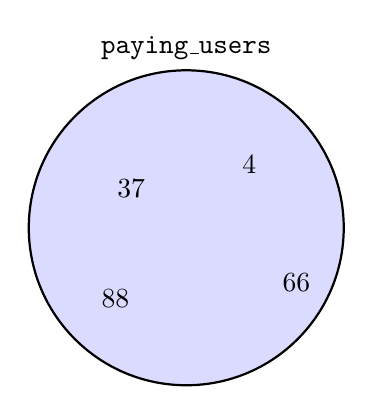
\begin{tikzpicture}[thick]
	\draw[fill={blue!35},fill opacity=0.4,text opacity=1] (0,0) circle (2)
		node[font=\ttfamily,above,shift={(0,2)}] { paying\_users };
	\node at (-0.9,-0.9) {$88$};
	\node at (1.4,-0.7) {$66$};
	\node at (0.8,0.8) {$4$};
	\node at (-0.7,0.5) {$37$};
\end{tikzpicture}
\end{center}

Successivamente, vengono aggiunti $2$ elementi all'insieme. Uno però, il $37$, è già presente,
quindi il numero di sringhe univoche aggiunte è solo $1$, come restituito dal comando.

\begin{center}
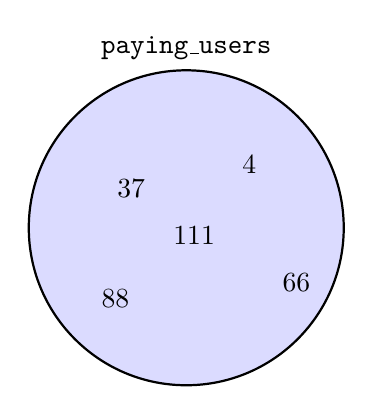
\begin{tikzpicture}[thick]
	\draw[fill={blue!35},fill opacity=0.4,text opacity=1] (0,0) circle (2)
		node[font=\ttfamily,above,shift={(0,2)}] { paying\_users };
	\node at (-0.9,-0.9) {$88$};
	\node at (1.4,-0.7) {$66$};
	\node at (0.8,0.8) {$4$};
	\node at (-0.7,0.5) {$37$};
	\node at (0.1,-0.1) {$111$};
\end{tikzpicture}
\end{center}

Il test di appartenenza dell'elemento $111$ tramite \cverb|SISMEMBER| \lnnum{2} restituisce $1$ per 
indicare che l'elemento è presente. Dopodiché, l'elemento $37$ viene rimosso dall'insieme tramite
\cverb|SREM| \lnnum{3}, e i successivi comandi \cverb|SCARD| e \cverb|ISMEMBER| confermano 
rispettivamente la nuova cardinalità dell'insieme ($4$) e l'assenza dell'elemento appena rimosso.

\begin{center}
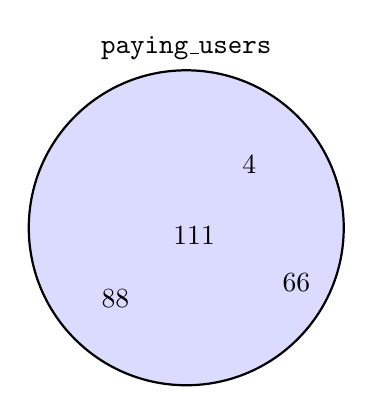
\begin{tikzpicture}[thick]
	\draw[fill={blue!35},fill opacity=0.4,text opacity=1] (0,0) circle (2)
		node[font=\ttfamily,above,shift={(0,2)}] { paying\_users };
	\node at (-0.9,-0.9) {$88$};
	\node at (0.8,0.8) {$4$};
	\node at (1.4,-0.7) {$66$};
	\node at (0.1,-0.1) {$111$};
\end{tikzpicture}
\end{center}

A questo punto, l'esempio crea un nuovo insieme \lnnum{4}: 

\medskip
\begin{center}
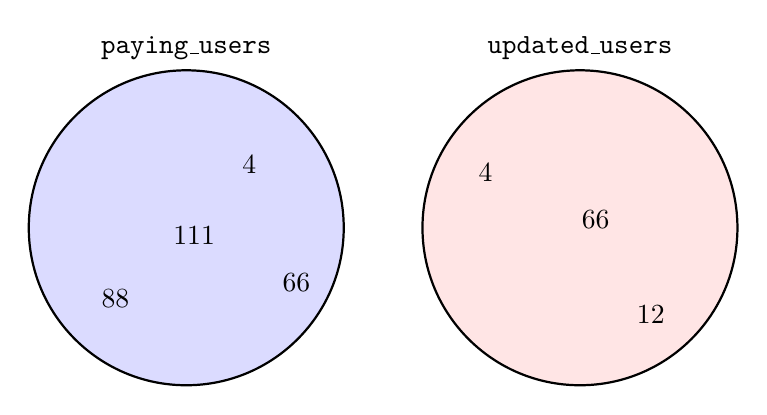
\begin{tikzpicture}[thick]
	\draw[fill={blue!35},fill opacity=0.4,text opacity=1] (-2.5,0) circle (2)
		node[font=\ttfamily,above,shift={(0,2)}] { paying\_users };
	\node at (-3.4,-0.9) {$88$};
	\node at (-1.7,0.8) {$4$};
	\node at (-1.1,-0.7) {$66$};
	\node at (-2.4,-0.1) {$111$};

	\draw[fill={red!25},fill opacity=0.4,text opacity=1] (2.5,0) circle (2)
		node[font=\ttfamily,above,shift={(0,2)}] { updated\_users };
	\node at (2.7,0.1) {$66$};
	\node at (3.4,-1.1) {$12$};
	\node at (1.3,0.7) {$4$};
\end{tikzpicture}
\end{center}

e ne calcola rispettivamente l'intersezione tramite \cverb|SINTER| \lnnum{5} e la differenza
tramite \cverb|SDIFF| \lnnum{6}:

\medskip
\begin{center}
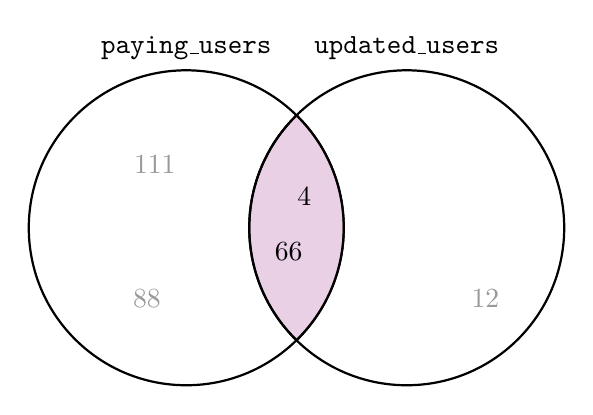
\begin{tikzpicture}[thick]
	\begin{scope}
		\clip {(1.4,0) circle (2)};
		\draw[fill={blue!35},fill opacity=0.4,text opacity=1] (-1.4,0) circle (2);
	\end{scope}
	\begin{scope}
		\clip {(-1.4,0) circle (2)};
		\draw[fill={red!25},fill opacity=0.4,text opacity=1] (1.4,0) circle (2);
	\end{scope}

	\draw(-1.4,0) circle (2) node[font=\ttfamily,above,shift={(0,2)}] { paying\_users };
	\node[text opacity=0.4] at (-1.9,-0.9) {$88$};
	\node[text opacity=0.4] at (-1.8,0.8) {$111$};

	\draw(1.4,0) circle (2) node[font=\ttfamily,above,shift={(0,2)}] { updated\_users };
	\node[text opacity=0.4] at (2.4,-0.9) {$12$};
	\node at (-0.1,-0.3) {$66$};
	\node at (0.1,0.4) {$4$};
\end{tikzpicture}
\end{center}
\medskip
\begin{center}
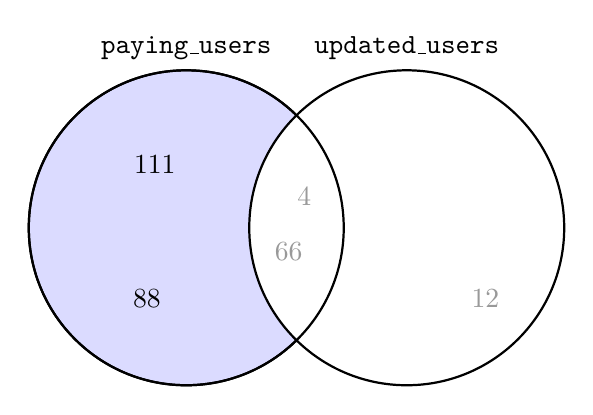
\begin{tikzpicture}[thick]
	\draw[fill={blue!35},fill opacity=0.4,text opacity=1] (-1.4,0) circle (2)
		node[font=\ttfamily,above,shift={(0,2)}] { paying\_users };
	\node at (-1.9,-0.9) {$88$};
	\node at (-1.8,0.8) {$111$};

	\draw[fill=white] (1.4,0) circle (2)
		node[font=\ttfamily,above,shift={(0,2)}] { updated\_users };
	\draw(-1.4,0) circle (2);
	\node[text opacity=0.4] at (2.4,-0.9) {$12$};
	\node[text opacity=0.4] at (-0.1,-0.3) {$66$};
	\node[text opacity=0.4] at (0.1,0.4) {$4$};
\end{tikzpicture}
\end{center}

\subsection{Insiemi ordinati}

Un insieme ordinato è una sequenza di stringhe univoche, ordinate secondo un valore associato
chiamato ``punteggio''. Ogni inserimento di una stringa viene effettuato specificando il suo
punteggio (aggiornando quindi un eventuale punteggio già esistente), e la struttura dati effettua
l'inserimento (o lo spostamento) nel modo giusto per mantenere l'ordinamento. In questo modo, è
possibile effettuare sia operazioni di tipo insiemistico (controllo appartenenza, aggiunta,
rimozione, unioni, intersezioni), sia operazioni che lavorano su intervalli di stringhe all'interno
della sequenza (per esempio, delimitandone gli estremi per punteggio).

Il punteggio deve essere specificato come un valore decimale con virgola, e le stringhe vengono
ordinate secondo l'ordinamento crescente. In caso due stringhe abbiano lo stesso punteggio, si
utilizza l'ordinamento lessicografico tra le stringhe stesse per deciderne l'ordine. In virtù di
questa proprietà, è comune utilizzare un insieme ordinato in cui tutti i valori hanno un medesimo
punteggio (di solito 0), utilizzando quindi le stringhe stesse per l'ordinamento, e ottenendo di
fatto l'equivalente di una lista di stringhe univoche ordinate alfabeticamente.

Come precedentemente accennato, è possibile estrarre sotto\-se\-quen\-ze dell'insieme ordinato tramite
alcuni comandi che lavorano su intervalli ordinati di stringhe. Secondo il principio di massima
flessibilità, ci sono tre diversi tipi di intervalli che possono essere specificati: intervallo di
punteggio (es: estrai tutte le stringhe i cui punteggi sono compresi tra 10 e 20), intervallo di
posizione (es: estrai le prime 10 stringhe secondo l'ordinamento attuale), oppure intervallo
lessicografico (es: estrai tutte le stringhe che iniziano con la lettera K); quest'ultimo tipo di
intervallo è in realtà correttamente definito solo quando il punteggio di tutte le stringhe è lo
stesso, e cioè quando la struttura dati sta di fatto già ordinando alfabeticamente, ma l'esistenza
di comandi dedicati a questa modalità sottolinea proprio la flessibilità di questa struttura dati.

Questi sono i principali comandi esistenti, identificati dal prefisso~\cverb|Z|:

\begin{description}[style=nextline,font={\bfseries\ttfamily}]
	\item[{ZADD key score ele [score ele\dots]}] Aggiunge una o più elementi (stringhe) all'insieme
		ordinato, associandole ad uno o più punteggi. Se le stringhe esistono già, il punteggio
		viene aggiornato al valore specificato. Il comando prevede anche una serie di opzioni
		avanzate per cambiare il comportamento in caso di stringa già esistente.
	\item[{ZINCRBY key incr ele}] Si comporta come \cverb|ZADD|, ma in caso di elemento esistente il
		punteggio viene modificato in modo relativo, sommando cioè il valore specificato invece che
		sostituirlo.
	\item[{ZREM key ele [ele\dots]}] Rimuove una o più stringhe dall'insieme, e restituisce il
		numero di elementi effettivamente rimossi.
	\item[ZSCORE key ele] Restituisce il punteggio associato ad un elemento, oppure \cverb|<nil>|
	    se l'elemento non esiste. Questo comando può quindi essere usato anche come test di
	    appartenenza.
	\item[ZCARD key] Restituisce la cardinalità dell'insieme, cioè il numero di
		stringhe contenute.
	\item[{ZINTERSTORE / ZUNIONSTORE dest numkeys key [key\dots] [WEIGHTS weight [weight\dots]]
		[AGGREGATE SUM|MIN|MAX]}] Come le controparti per gli insiemi, effettuano le operazioni
		(rispettivamente) di unione e intersezione, memorizzando il risultato in un nuovo insieme
		ordinato. Il punteggio ottenuto è la somma dei punteggi specificati negli insiemi di
		origine, ma è possibile specificare una funzione di aggregazione diversa (media, minimo o
		massimo) tramite l'opzione \cverb|AGGREGATE|, ed applicare dei pesi (fattori moltiplicativi)
		ai punteggi tramite l'opzione \cverb|WEIGHTS|.
	\item[ZRANGE key start stop] Restituisce gli elementi all'interno dell'intervallo
		specificato come indice di sequenza. Per esempio, specificando come intervallo inclusivo
		\cverb|0 4|, si ottengono i primi 5 elementi, cioè i 5 elementi con minor punteggio
		attualmente presenti nell'insieme. È possibile usare gli indici negativi per fare
		riferimento alla fine della sequenza (per esempio, \cverb|-1| indica l'elemento con
		punteggio più alto).
	\item[{ZRANGEBYSCORE key min max [LIMIT offset count]}] Restituisce gli elementi all'interno
		dell'intervallo specificato come punteggi. Per esempio, specificando come intervallo
		\cverb|100.2 100.8|, si ottengono tutti gli elementi i cui punteggi sono $\in
		\interval{100.2}{100.8}$. Gli estremi dell'intervallo si intendo chiusi, ma possono essere
		specificati come aperti tramite il prefisso \cverb|(|: per esempio \cverb|5.4 (8|
		indica l'intervallo $\interval[open right]{5.4}{8}$. È possibile inoltre specificare un
		numero massimo di elementi restituiti tramite l'opzione \cverb|LIMIT|, per evitare
		trasferimenti troppo pesanti, consentendo quindi la paginazione.
	\item[{ZRANGEBYLEX key min max [LIMIT offset count]}] Restituisce gli elementi all'interno
		dell'intervallo specificato come prefissi lessicografici. Per esempio, specificando come
		intervallo \cverb|AZ C|, si ottengono tutti gli elementi che seguono lessicograficamente
		la stringa ``AZ'' e precedono la stringa ``C''. Come per il comando precedente, è possibile
		specificare se gli estremi dell'intervallo sono aperti o chiusi, e indicare un limite
		massimo agli elementi restituiti. Come già descritto, questo comando funziona correttamente
		solo con insiemi ordinati in cui tutti gli elementi hanno lo stesso punteggio.
	\item[ZREVRANGE / ZREVRANGEBYSCORE / ZREVRANGEBYLEX] Simili ai precedenti comandi, ma
		considerano l'insieme ordinato al contrario, cioè in ordine decrescente di punteggio.
	\item[ZREMRANGEBYRANK / ZREMRANGEBYSCORE / ZREMRANGEBYLEX] Simili ai precedenti comandi, ma
		rimuovono gli elementi all'interno degli intervalli specificati invece che restituirli.
\end{description}

Anche gli insiemi ordinati, come gli insiemi, si prestano molto bene a creare indici manuali,
sempre ordinati, su cui effettuare poi operazioni di estrazione e ricerca. Vista la flessibilità
della struttura dati, indichiamo alcuni possibili scenari applicativi.

\begin{itemize}
	\item Un esempio di struttura dati facilmente rappresentabile tramite insieme ordinato è una
	coda con priorità. Supponiamo per esempio di dover memorizzare un elenco di azioni da eseguire
	nel futuro, assieme con l'istante temporale al quale l'azione deve essere eseguita. Al momento
	di inserire un'azione, si può creare un nuovo elemento in una tabella hash (\cverb|HSET|)
	utilizzando un ID progressivo conservato in una chiave (\cverb|INCR|), memorizzando così tutto
	il dettaglio dell'azione da eseguire (tipologia, parametri, condizioni di errore). Dopodiché,
	si inserisce l'ID dell'azione in un insieme ordinato (\cverb|ZADD|), utilizzando come punteggio
	il timestamp UNIX a cui si dovrà eseguire l'azione. Successivamente, in polling, è possibile
	estrarre tutte le azioni scadute (cioè il cui timestamp è inferiore all'attimo corrente,
	tramite \cverb|ZRANGEBYSCORE|) e processarle; via via che ciascuna azione termina l'esecuzione,
	può essere rimossa dall'insieme (\cverb|ZREM|).

	\item Supponiamo di voler creare un sistema di fidelizzazione per un e-commerce, basato sulla
	spesa effettuata da ciascun utente. Ogni volta che un utente effettua un acquisto, possiamo
	inserirlo nell'insieme ordinato l'ID dell'utente aggiungendo l'importo del carrello
	(\cverb|ZINCR|); non è necessario gestire in modo diverso il primo acquisto, perché \cverb|ZINCR|
	funziona anche se l'elemento non è ancora presente. Se vogliamo contattare tutti gli utenti che
	hanno speso più di \SI{1000}{\EUR} sul nostro e-commerce, possiamo utilizzare
	\cverb|ZRANGEBYSCORE| specificando l'intervallo $\interval{1000.00}{\infty}$ (tramite la stringa
	\cverb|1000.00 +inf|) per estrarre gli ID. In alternativa, supponendo di voler premiare i
	$100$ utenti che hanno speso di più, possiamo estrarre i loro ID con \cverb|ZREVRANGE| usando
	l'intervallo \cverb|0 99| (essendo l'insieme in ordine crescente, dobbiamo usare
	\cverb|ZREVRANGE| per estrarre facilmente gli elementi con punteggio più grosso).
\end{itemize}

Qui si può vedere una semplice sessione interattiva di esempio di uso degli insiemi ordinati:

\begin{commentedsource}[style=redis]
|\lnote|127.0.0.1:6379> ZADD paying_users 2500 tim 800 max 1000 sam 
(integer) 3
127.0.0.1:6379> ZADD paying_users 3000 tim 500 peg
(integer) 1
|\lnote|127.0.0.1:6379> ZCARD paying_users
(integer) 4
|\lnote|127.0.0.1:6379> ZINCRBY paying_users 1200 max
"2000"
127.0.0.1:6379> ZSCORE paying_users max
"2000"
|\lnote|127.0.0.1:6379> ZRANGE paying_users 0 1
1) "peg"
2) "sam"
127.0.0.1:6379> ZREVRANGE paying_users 0 1 WITHSCORES
1) "tim"
2) "3000"
3) "max"
4) "2000"
|\lnote|127.0.0.1:6379> ZRANGEBYSCORE paying_users 1500 2500
1) "max"
127.0.0.1:6379> ZINCRBY paying_users 2000 max
"4000"
127.0.0.1:6379> ZRANGEBYSCORE paying_users 1500 2500
(empty list or set)
|\lnote|127.0.0.1:6379> ZRANGEBYSCORE paying_users 3000 (4000
1) "tim"
\end{commentedsource}

Inizialmente, viene creato un insieme ordinato \cverb|paying_users| contenente 3 elementi \lnnum{1};
poiché l'insieme è ordinato, rappresentiamo i dati rispettando subito il punteggio associato a
ciascun elemento:

\begin{center}
	\begin{tabular}{|*{3}{c|}}
	  \hline
	  \cellcolor{blue!25}{\num{800}} & \cellcolor{blue!25}{\num{1000}} & \cellcolor{blue!25}{\num{2500}} \\ 
	  \cellcolor{blue!25}{max} & \cellcolor{blue!25}{sam} & \cellcolor{blue!25}{tim} \\ 
	  \hline
	\end{tabular}
\end{center}

Il successivo comando \cverb|ZADD| aggiunge due elementi: l'elemento \cverb|tim| però era già
presente nell'insieme, e quindi il suo punteggio viene aggiornato:

\begin{center}
	\begin{tabular}{|*{4}{c|}}
	  \hline
	  \cellcolor{blue!25}{\num{500}} & \num{800} & \num{1000} & \cellcolor{blue!25}{\num{3000}} \\ 
	  \cellcolor{blue!25}{peg} & max & sam & \cellcolor{blue!25}{tim} \\ 
	  \hline
	\end{tabular}
\end{center}

Infatti, si può verificare che la nuova cardinalità è $4$ \lnnum{2}.

Il comando \cverb|ZINCRBY| \lnnum{3} modifica il punteggio dell'elemento \cverb|max|,
incrementandolo di $800$, e restituisce il nuovo punteggio $2000$. Il punteggio può anche
essere estratto tramite \cverb|ZSCORE|, per verificarne il valore corrente.

\begin{center}
	\begin{tabular}{|*{4}{c|}}
	  \hline
	  \num{500} & \num{1000} & \cellcolor{blue!25}{\num{2000}} & \num{3000} \\ 
	  peg & sam & \cellcolor{blue!25}{max} & tim \\ 
	  \hline
	\end{tabular}
\end{center}

Per estrarre porzioni di contenuto dell'insieme, viene utilizzato \cverb|ZRANGE| con un intervallo
che indica l'elemento di inizio e quello di fine dell'estrazione da effettuare, in ordine di
punteggio; per esempio \cverb|0 1| indica i 2 elementi con valore più basso \lnnum{4}. Il comando
\cverb|ZREVRANGE| si comporta nello stesso modo, ma estrae elementi partendo dal fondo dell'insieme,
cioè in ordine inverso di punteggio. L'opzione \cverb|WITHSCORES| specifica di estrarre anche
i punteggi oltre agli elementi.

Il comando \cverb|ZRANGEBYSCORE| effettua un'estrazione utilizzando non più indici, ma un range di
punteggi. Specificando \cverb|1500 2500| \lnnum{5}, l'unico elemento compreso in questo intervallo è
\cverb|max|, che viene restituito. Se si aumenta il punteggio di \cverb|max| portandolo a $4000$,
una seconda invocazione di \cverb|ZRANGEBYSCORE| sul medesimo intervallo non restituisce più
alcun elemento.

\begin{center}
	\begin{tabular}{|*{4}{c|}}
	  \hline
	  \num{500} & \num{1000} & \num{3000} & \cellcolor{blue!25}{\num{4000}} \\ 
	  peg & sam & tim & \cellcolor{blue!25}{max} \\ 
	  \hline
	\end{tabular}
\end{center}

Come ultimo caso, si noti l'uso dell'identificatore speciale \cverb|(| per indicare un intervallo
aperto: specificando l'intervallo \cverb|3000 (4000|, corrispondente a 
$\interval[open right]{3000}{4000}$, il solo elemento \cverb|tim| viene restituito, poiché \cverb|max|
è escluso dall'intervallo.

\subsection{HyperLogLog}

HyperLogLog \cite{hyperloglog} è una struttura dati probabilistica con la quale è possibile
calcolare in modo efficiente il numero di elementi distinti di un multi-insieme. 

Normalmente, per poter contare elementi distinti, è necessario memorizzare tutti gli elementi visti
almeno una volta, in modo da scartare i duplicati (utilizzando quindi un insieme), e ricavare infine
la cardinalità. Questa implementazione però utilizza una quantità di memoria proporzionale al numero
di elementi distinti, che può essere quindi molto elevata quando gli elmenti sono milioni o
miliardi. HyperLogLog invece richiede una frazione dello spazio, in base a come è configurato: per
esempio, nell'implementazione di Redis la memoria occupata da ciascun HyperLogLog è pari a
\SI{12}{\kibi\byte}, indipendentemente dalla quantità di dati conteggiati, e l'errore standard della
cardinalità calcolata è pari allo \SI{0.83}{\percent}.

Rimandando a \cite{hyperloglog} per una trattazione approfondita, l'intuizione base di HyperLogLog,
come spiegato in \cite{hyperloglog-explain}, è che, osservando nella loro rappresentazione binaria
un multi-insieme di numeri equamente distribuiti, se troviamo uno specifico prefisso di $N$ bit
predeterminato, è possibile ipotizzare che la cardinalità dell'insieme sia almeno $2^N$; per
esempio, in un insieme di numeri casuali, circa il \SI{12.5}{\percent} di essi ha un prefisso
binario pari a \cverb|001|, per cui se troviamo questo prefisso, possiamo ipotizzare che i numeri
siano almeno \num{8}. Effettuando questo test con prefissi sempre più lunghi (cercando cioè, il più
lungo prefisso di zeri iniziali nel multi-insieme), è possibile ottenere una stima della
cardinalità.

Questa osservazione però commette un errore con varianza molto elevata, per cui HyperLogLog divide i
numeri in ingresso in più sottoinsiemi, effettua per ciascuno una stima della cardinalità e poi
bilancia queste stime tramite una media armonica. Per ciascun sottoinsieme, è sufficiente quindi
conservare un registro, che conti il prefisso più lungo visto. Si calcola che l'errore standard 
risultante è pari a $1.04 / \sqrt{m}$, con $m$ pari al numero di registri. 

Per distribuire uniformemente le stringhe in input, Redis utilizza una funzione di hash a
\SI{64}{\bit} (come suggerito in \cite{hyperloglog-plusplus}), in particolare scegliendo
MurMurHash64, una versione a \SI{64}{\bit} del già citato
\fnhref{https://github.com/aappleby/smhasher/wiki/MurmurHash3}{MurMurHash3}. Essendo quindi il
prefisso massimo lungo appunto 64 bit, i registri richiedono 6 bit. Redis sceglie di usare $2^{14}$
registri, ottenendo quindi un errore pari a $1.04 / \sqrt{2^{14}} = \SI{0.8}{\percent}$, e
utilizzando un totale di $2^{14} * 6 / 8 = \num{12228}$ byte di memoria necessaria, come già
riportato.

Questi sono i comandi esistenti, identificati dal prefisso~\cverb|PF|:

\begin{description}[style=nextline,font={\bfseries\ttfamily}]
	\item[PFADD] Aggiunge una o più stringhe all'HyperLogLog spe\-ci\-fi\-ca\-to,
	creandone uno se non esiste già.
	\item[PFCOUNT] Restituisce l'attuale stima di cardinalità dell'HyperLogLog
	specificato.
	\item[PFMERGE] Fonde due o più HyperLogLog, creando un nuovo HyperLogLog che
	stima la cardinalità dell'unione degli insiemi specificati.
\end{description}

Un tipico caso d'uso è quello di conteggiare i cosiddetti \emph{DAU}, ``daily active users'', cioè
il numero di utenti attivi in un'applicazione all'interno di ciascuna giornata solare.
L'applicazione, alla mezzanotte, può creare un nuovo HyperLogLog utilizzando una chiave derivata dal
giorno in corso (per esempio, \cverb|DAU-2017-09-02|), aggiungendo via via l'ID di ciascun utente
(tramite \cverb|PFADD|) ogni volta che ne viene rilevata una qualunque attività, senza doversi
preoccupare di tenere conto se l'utente era già stato conteggiato come attivo o meno. Al termine
della giornata, è possibile stimare i \emph{DAU} tramite il comando \cverb|PFCOUNT|. Lo storico può
essere conservato per ragioni di analisi a posteriori, e può essere aggregato tramite
\cverb|PFMERGE| per ottenere stime di attività su finestre temporali diverse, per esempio su base
settimanale o mensile (cosiddetti rispettivamente \emph{WAU} o \emph{MAU}). Grazie all'HyperLogLog,
l'utilizzo di memoria è costante indipendentemente dal numero di utenti attivi, anche se questi
dovessero raggiungere importanti volumi; a titolo di esempio, il numero di \emph{MAU} su Facebook in
Giugno 2017 è stato più di 2 miliardi \cite{fb-mau}.

Qui si può vedere una sessione interattiva di esempio di uso di HyperLogLog:

\begin{commentedsource}[style=redis]
|\lnote|127.0.0.1:6379> PFADD dau 50
(integer) 1
127.0.0.1:6379> PFCOUNT dau
(integer) 1
|\lnote|127.0.0.1:6379> PFADD dau 51 52 50 53 54 50 55 56 50 57 58 59 50
(integer) 1
127.0.0.1:6379> PFCOUNT dau
(integer) 10
|\lnote|127.0.0.1:6379> PFADD dau 51 52 53 54 55 56 57 58 59 61
(integer) 1
127.0.0.1:6379> PFCOUNT dau
(integer) 11
\end{commentedsource}

Inizialmente, viene aggiunto il valore $50$ all'HyperLogLog denominato \cverb|dau| \lnnum{1} (che
viene quindi creato con questo primo comando), e successivamente si può verificare che la
cardinalità dell'insieme è al momento quella attesa, cioè $1$.

Vengono poi aggiunti un gruppo di valori \lnnum{2} di cui alcuni non già presenti (i numeri dal $51$
al $59$) ma altri invece già presenti (il numero $50$, che viene aggiunto per 3 volte nella
sequenza, pur essendo già presente). La cardinalità però risulta comunque corretta: infatti
\cverb|PFCOUNT| restituisce il valore atteso $10$, visto che in questo momento nella struttura sono
stati inseriti tutti i valori tra il $50$ e il $59$. 

Infine, si prova nuovamente ad inserire un insieme di valori \lnnum{3} tutti già visti tranne
l'ultimo ($61$). La cardinalità ancora una volta è corretta, poiché misura $11$, avendo scartato
correttamente i valori già visti e aggiunto solo l'elemento $61$.

\section{Transazioni}

Nella teoria delle basi di dati, una transazione è una sequenza di operazioni disgiunte che
modificano la base di dati in modo corretto solo se eseguite accorpate, come fossero una singola
operazione. Le proprietà che un sistema di transazioni può offrire sono 4: atomicità (la transazione
viene eseguita nel suo complesso, oppure fallisce senza che nessun risultato parziale sia visibile),
coerenza (vengono rispettati i vincoli di integrità all'inizio e alla fine della transazione),
isolamento (durante l'esecuzione di una transizione, lo stato che essa osserva della base di dati
non deve essere modificato da operazioni che avvengono parallelamente), e durabilità (una
transazione eseguita con successo modifica la base di dati in modo persistente, senza cioè che la
modifica possa più essere persa a causa di un arresto anomalo). Queste proprietà vengono comunemente
chiamate tramite il loro acronimo ACID, e un database è detto supportare transazioni ACID se espone
un sistema di transazioni che verifichino contemporaneamente le 4 proprietà.

Il supporto per le transazioni di Redis è molto primitivo: è possibile infatti raggruppare
una sequenza di comandi in modo che venga eseguita atomicamente dal server, senza possibilità che
altre operazioni (eseguite da altri client) possano inframezzarsi. Non è però previsto nessun
meccanismo di ripristino in caso uno dei comandi inviati fallisca: la transazione si interrompe
semplicemente restituendo il codice di errore del comando, ma senza annullare le modifiche
eventualmente operate dai comandi precedenti.

Per utilizzare una transazione, è sufficiente inviare il comando \cverb|MULTI|, seguito dalla 
sequenza di comandi che si vuole eseguire atomicamente, seguiti dal comando \cverb|EXEC|, che dà
il via all'esecuzione. I valori di ritorno di tutti i comandi vengono concatenati e restituiti come
valore di ritorno del comando \cverb|EXEC|. È possibile anche annullare una transazione prima di
eseguirla, inviando il comando \cverb|DISCARD|. Vediamo un esempio:

\begin{commentedsource}[style=redis]
127.0.0.1:6379> HMSET user:123 name Giovanni surname Bajo
OK
|\lnote|127.0.0.1:6379> ZADD paying-users 1500 123
(integer) 1
127.0.0.1:6379> HMSET user:124 name Mickey surname Mouse
OK
|\lnote|127.0.0.1:6379> ZADD paying-users 1200 124
(integer) 1
127.0.0.1:6379> MULTI
OK
127.0.0.1:6379> DEL user:123
|\lnote|QUEUED
127.0.0.1:6379> ZREM paying-users 123
|\lnote|QUEUED
|\lnote|127.0.0.1:6379> EXEC
1) (integer) 1
2) (integer) 1
\end{commentedsource}

All'inizio, viene create una tabella hash per memorizzare i record relativi agli utenti (tramite
\cverb|HMSET|) e un insieme ordinato che rappresenta un indice della tabella (\cverb|paying-users|,
tramite \cverb|ZADD|). Il primo utente ha ID $123$, e ha speso un totale di \SI{1500}{\EUR}
\lnnum{1}, mentre il secondo utente con ID $124$ ha speso \SI{1200}{\EUR} \lnnum{2}.

L'esempio mostra quindi come rimuovere atomicamente l'utente con ID $123$: viene utilizzata una
transazione per evitare che altri client possano accedere ad uno stato inconsistente nel quale
l'utente è presente come record ma non nell'indice (o viceversa). Durante la transazione,
vengono eseguiti i comandi \cverb|DEL| e \cverb|ZREM| per rimuovere l'utente sia dalla tabella
hash sia dall'indice, e il valore di ritorno \cverb|QUEUED| \lnnum{3} \lnnum{4} mostra come
i comandi non sono stati eseguiti immediatamente, ma accodati in attesa della fine della 
definizione della transazione, delimitata dal comando \cverb|EXEC| \lnnum{5}.

Relativamente alle proprietà ACID sopra descritte, è possibile osservare che:

\begin{itemize}
	\item \textbf{Atomicità}: la proprietà non viene rispettata, poiché se un comando all'interno
	delle transazione fallisce, la transazione viene bloccata a metà della propria esecuzione,
	ma senza effettuare un ripristino del database allo stato iniziale. Si noti inoltre che i
	comandi di Redis tipicamente non restituiscono errori su chiavi non trovate o non esistenti, 
	preferendo restituire valori speciali come numeri negativi; in questi casi, la transazione
	continua. 

	\item \textbf{Coerenza}: questa proprietà non si applica a Redis perché non è possibile definire 
	veri vincoli d'integrità nella base di dati.

	\item \textbf{Isolamento}: la proprietà viene rispettata perché l'esecuzione dei comandi
	della transazione è perfettamente isolata da altri client, che rimangono in attesa. Questo
	comportamento è ottenuto semplicemente tramite l'approccio a singolo thread di esecuzione (si
	veda la \autoref{sec:concurrency} per maggiori informazioni).

	\item \textbf{Durabilità}: questa possibilità può essere rispettata se Redis viene configurato
	per effettuare una piena persistenza dei dati dopo ciascun comando. Questa possibilità
	verrà dettagliata nella	\autoref{sec:durability:aof}.
\end{itemize}


\subsection{Transazioni condizionali}

Come appena descritto, il sistema di transazioni di Redis si basa su accodare comandi ed eseguirli
poi sequenzialmente in modo atomico; ma, poiché qualunque comando viene accodato, non è possibile
inviare un comando i cui parametri dipendono da valori restituiti da comandi precedenti; infatti il
client non avrà accesso al valore di ritorno di un comando fino a che l'intera transazione non sarà
stata eseguita, né è disponibile una sintassi speciali per referenziare il valore restituito da un
comando precedente.

Supponiamo di implementare un social network e di voler incrementare in modo atomico un campo
memorizzato all'interno di una tabella hash, per esempio il numero di commenti che un determinato
post ha ricevuto; poiché il comando \cverb|INCR| agisce solo su chiavi di tipo stringa, e non quindi
su campi di una tabella hash, sarà necessario utilizzare il comando \cverb|HGET| per estrarre il
valore corrente \lnnum{1}, e poi \cverb|HSET| per inserire il nuovo valore incrementato \lnnum{2}, in
questo modo:

\begin{commentedsource}[style=redis]
|\lnote|127.0.0.1:6379> HGET post:589 vote
"56"
|\lnote|127.0.0.1:6379> HSET post:589 vote 57
(integer) 0
\end{commentedsource}

Purtroppo questa sequenza è soggetta ad una \emph{race condition} da parte di un altro client che
volesse modificare lo stesso campo. Non sembra inoltre possibile utilizzare una transazione basata
su \cverb|MULTI| e \cverb|EXEC| perché il comando \cverb|HSET| può essere inviato dal client solo dopo
che ha ricevuto la risposta al comando \cverb|HGET|:

\begin{commentedsource}[style=redis]
127.0.0.1:6379> MULTI
OK
127.0.0.1:6379> HGET post:589 vote
|\lnote|QUEUED
|\lnote|127.0.0.1:6379> HSET post:589 ???
\end{commentedsource}

Poiché il comando \cverb|HGET| è stato accodato in attesa del termine della transazione, il client
non ha ricevuto il valore del campo richiesto \lnnum{1}, e non è quindi in grado di sapere quale
nuovo valore inserire \lnnum{2}.

Per risolvere queste situazioni, Redis utilizza un comune pattern di transazione atomica chiamato
``check and set'', che consente di condizionare l'esecuzione di una transazione alla verifica che un
valore non sia mutato rispetto a quanto atteso. Il comando \cverb|WATCH| infatti consente di
annullare automaticamente una transazione se il valore di una chiave cambia tra il momento in cui
viene eseguito e il momento in cui la transazione viene eseguita, cioè se si è effettivamente
verificata una race condition. In questo caso, il client vorrà probabilmente provare nuovamente ad
eseguire la transazione, nella speranza di riuscire a vincere la corsa.

Questo è l'uso corretto di \cverb|WATCH| nell'esempio che stiamo a\-na\-liz\-zan\-do:

\begin{commentedsource}[style=redis]
|\lnote|127.0.0.1:6379> WATCH post:589
OK
127.0.0.1:6379> HGET post:589 vote
|\lnote|"56"
127.0.0.1:6379> MULTI
OK
|\lnote|127.0.0.1:6379> HSET post:589 vote 57
QUEUED
127.0.0.1:6379> EXEC
1) (integer) 0
\end{commentedsource}

In questo caso, dopo aver attivata l'osservazione della chiave con \cverb|WATCH| \lnnum{1}, il
comando di lettura viene eseguito prima della transazione, ricevendo quindi il valore
attuale del campo richiesto \lnnum{2}, che può essere incrementato e modificato durante la transazione
\lnnum{3}.

Vediamo cosa succede invece simulando l'intervento di un client esterno che modifica il valore
del post in modo concorrente:

\begin{commentedsource}[style=redis]
127.0.0.1:6379> WATCH post:589
OK
|\lnote|127.0.0.1:6379> HGET post:589 vote
"56"
|\lnote|127.0.0.1:6379> HSET post:589 vote 57
(integer) 0
127.0.0.1:6379> MULTI
OK
127.0.0.1:6379> HSET post:589 vote 57
QUEUED
127.0.0.1:6379> EXEC
|\lnote|(nil)
\end{commentedsource}

In questo caso, l'esempio simula una modifica \lnnum{2} effettuata dopo la lettura della chiave
\lnnum{1}, come se fosse stata fatta da un altro client in modo concorrente; questa modifica fa sì
che la transazione non venisse eseguita e fosse annullata: il client può rilevare questa condizione
dal valore restituito da \cverb|EXEC| (che è \cverb|nil| \lnnum{3}, invece che un array contenente i
valori restituiti dai comandi della transazione), e riprovare nuovamente la sequenza.

\section{Velocità}

(benchmark)
(segnalare problema del rountrip di rete)


\section{Pipelining}

Come dettagliato nella precedente sessione, le prestazioni ottenute nell'utilizzo di Redis sono
fortemente influenzate dalla velocità di rete. Sebbene le migliori pratiche di installazione in
ambiente di produzione consigliano di posizionare rete su un server (o gruppi di server) fisicamente
vicini al server dove girare l'applicazione client, in popolari ambienti cloud come Amazon Web
Services è possibile misurare latenze anche nell'ordine di \SI{50}{\milli\second} se si considerano
misure al 99-esimo percentile, sebbene con valori mediani stabilmente sotto il millisecondo
\cite{aws-latency}.

L'utilizzo di transazioni, sebbene utile per introdurre il concetto di atomicità di esecuzione,
non migliora la latenza poiché ogni comando viene inviato separatamente e necessita quindi di un 
roundtrip (ai quali si sommano addirittura i due roundtrip richiesti da \cverb|MULTI| e \cverb|EXEC|).

Per arginare questo problema, Redis consente il \emph{pipelining}, una tecnica molto comune, 
utilizzata anche da altri protocolli di tipo master-slave come HTTP, IMAP e POP3. Dopo l'invio 
di un comando, il client può immediatamente inviarne un secondo senza necessariamente leggere
la risposta del primo dalla rete; il server infatti è in grado di mantenere memorizzate le risposte
dei comandi (memoria permettendo) indefinitamente, in attesa che il client le richieda. Dovendo
quindi eseguire una sequenza predeterminata di comandi, come nel caso di una transazione, il
pipelining risulta particolarmente comodo perché l'intera transazione (comprensiva dei delimitatori
\cverb|MULTI| e \cverb|EXEC|) può essere inviata consecutivamente, praticamente senza attese.

\begin{figure}
	\centering
	\begin{minipage}[t]{0.4\textwidth}
		\subfloat[][Senza \emph{pipelining}]{
			\begin{sequencediagram}
			\newthread[green]{a}{:Client} \newthread[blue]{b}{:Server}
			\mess[2]{a}{}{b}
			\prelevel
			\mess[2]{b}{}{a}
			\prelevel
			\mess[2]{a}{}{b}
			\prelevel
			\mess[2]{b}{}{a}
			\prelevel
			\mess[2]{a}{}{b}
			\prelevel
			\mess[2]{b}{}{a}
			\end{sequencediagram}
		}
	\end{minipage}
	\qquad
	\begin{minipage}[t]{0.4\textwidth}
		\subfloat[][Con \emph{pipelining}]{
			\begin{sequencediagram}
			\newthread[green]{a}{:Client} \newthread[blue]{b}{:Server}
			\mess[2]{a}{}{b}
			\prelevel\prelevel
			\mess[2]{a}{}{b}
			\prelevel\prelevel
			\mess[2]{a}{}{b}
			\prelevel\prelevel\prelevel
			\mess[2]{b}{}{a}
			\prelevel\prelevel
			\mess[2]{b}{}{a}
			\prelevel\prelevel
			\mess[2]{b}{}{a}
			\postlevel\postlevel\postlevel\postlevel
			\postlevel\postlevel
			\end{sequencediagram}
		}
	\end{minipage}

	\caption{Diagramma di sequenza che mostra l'uso del \emph{pipelining} per diminuire
		il tempo totale d'e\-se\-cu\-zio\-ne di 3 comandi}
\end{figure}

Si noti che, se si è interessati ad ottenere la massima performance, è consigliabile anche
disattivare il controllo della congestione del TCP, descritto in
\cite{rfc896} (detto anche \emph{algoritmo di Nagle} dal nome
dell'autore), che rallenta l'invio di pacchetti piccoli di dati aggregandoli in ``segmenti'',
diminuendo il traffico sulla rete ma aumentando la latenza fino anche a \SI{500}{\milli\second}), ed
utilizzare le opzioni \cverb|TCP_NODELAY| e \cverb|TCP_CORK| per gestire manualmente il buffering
\cite{tcp-cork}. Molte librerie client Redis per i principali linguaggi di programmazione si
occupano di questi dettagli automaticamente; si veda a titolo di esempio i 
\fnhref{https://github.com/andymccurdy/redis-py/blob/8a186eb/redis/connection.py\#L517}{sorgenti della libreria \texttt{redis-py}}.

\section{Stored procedure in LUA}
\label{sec:redis:lua}

Il \emph{pipelining} non è però in grado di essere sempre utilizzato: per esempio, può essere
necessario verificare che un comando abbia successo prima di procedere al successivo; oppure
può essere necessario utilizzare il valore restituito da un comando per definire il parametro 
di un comando successivo. In questi casi, è necessario quindi introdurre un nuovo roundtrip di
rete per leggere la risposta, processarla, e inviare il successivo comando.

Esattamente come nel caso dei comuni database SQL, Redis consente di risolvere in modo più completo
il problema della latenza di rete tramite le cosiddette \emph{stored procedure}: il programmatore
può inviare al database un programma speciale, che viene memorizzato per usi successivi, ed
eseguirlo poi successivamente; questo programma può quindi effettuare più operazioni in successione,
oltre che utilizzare istruzioni per controllo di flusso, pagando, in termini di latenza, un solo
roundtrip di rete. Inoltre, specialmente nel caso in cui sia necessario effettuare delle funzioni di
aggregazione di dati (es: calcolo di una media), non è necessario trasferire via rete tutti i dati,
ma solamente il risultato.

Invece che utilizzare un linguaggio di programmazione progettato ad-hoc (come per esempio il
\fnhref{https://www.postgresql.org/docs/9.6/static/plpgsql.html}{linguaggio PL/pgSQL} utilizzato dal
famoso database PostgreSQL), Redis utilizza un linguaggio già esistente:
\fnhref{https://www.lua.org}{LUA}. LUA è un linguaggio di scripting, tipizzato dinamicamente,
normalmente eseguito tramite un interprete molto efficiente e compatto, facilmente adatto
all'integrazione (embedding). Già dai primi anni 2000, ha ottenuto popolarità nell'industria
di videogiochi come linguaggio di scripting, proprio in virtù del profilo di performance e
compatezza che lo rendeva utilizzabile anche all'interno di console con processori non troppo
potenti e quantitativi di memoria limitati (si pensi per esempio alla Sony Playstation 2, che era
comandata da un processore MIPS R5900 a \SI{300}{\mega\hertz} con \SI{32}{\mebi\byte} di RAM), ed è
stato utilizzato all'interno di successi quali Angry Birds \cite{lua-angry} o World of Warcraft
\cite{lua-wow}.

Supponiamo di voler scrivere una stored procedure che calcoli un dato statistico aggregato; per
esempio, dato un insieme ordinato \cverb|paying-users| in cui le stringhe sono gli ID degli utenti di
un sistema, e il punteggio associato è il totale speso dall'utente nell'applicazione, vogliamo
calcolare qual è la media di spesa degli utenti ``premium'', cioè che hanno speso più di
\SI{1000}{\EUR}. Per fare questo, è necessario estrarre prima la lista degli utenti ``premium''
tramite il comando \cverb|ZRANGEBYSCORE|, e poi iterare in questa lista calcolando il valore medio.
L'utilizzo di una stored precedure ci consente di fare questo senza trasferire sulla rete le
informazioni relative a tutti gli utenti ``premium'', che potrebbero essere migliaia o anche più. Il
sorgente LUA che implementa questo semplice algoritmo è mostrato nel seguente listato:

\medskip
\sourcecode[language={[5.0]lua}]{code/zsetaverage.lua}

Le stored procedure in Redis ricevono in ingresso due array di parametri che possono essere passati
dal chiamante: uno chiamato \cverb|KEYS| che contiene chiavi di oggetti nel database, e uno chiamato
\cverb|ARGV|, che contiene argomenti arbitrari di altro tipo. Nello script d'esempio, si è scelto di
passare come parametri il nome dell'insieme ordinato in \cverb|KEYS[1]|, e la soglia minima di spesa
in \cverb|ARGV[1]|, rendendo così lo script più generico e flessibile. Si noti che in Lua, gli array
sono indicizzata a partire da $1$, per cui \cverb|KEYS[1]| si riferisce al primo elemento 
dell'array.

Per provare ad eseguire lo script durante la fase di sviluppo, è consigliabile l'utilizzo
dell'opzione \cverb|--eval| del comando \cverb|redis-cli|:

\begin{commentedsource}[style=redis]
$ redis-cli
127.0.0.1:6379> ZADD paying_users 1000 a 2000 b 3000 c 3000 d 250 e
(integer) 5
|\lnote|$ redis-cli --eval zsetaverage.lua paying_users , 1000
(integer) 2250
$ redis-cli --eval zsetaverage.lua paying_users , 2000
(integer) 2666
\end{commentedsource}

Si noti che, a linea di comando, è necessario separare esplicitamente gli argomenti che
popolano \cverb|KEYS| da quelli che popolano \cverb|ARGV|, perché altrimenti non sarebbe chiaro
per Redis dove finiscono gli uni e iniziano gli altri. Il separatore da usare è l'identificatore 
\cverbfull|,|. Di conseguenza, usando la sequenza di argomento \cverb|paying_users , 1000|
\lnnum{1}, si popola in modo corretto gli array: \cverb|KEYS[1]| varrà \cverb|paying_users|, e
\cverb|ARGV[1]| varrà \cverb|1000|.

Vediamo un esempio di come usare invece una stored procedure in produzione:

\begin{commentedsource}[style=redis]
|\lnote|127.0.0.1:6379> SCRIPT LOAD "-- zsetaverage.lua: calcola la media di spesa degli utenti paganti sopra\n-- una certa soglia.\n--\n-- Argomenti:\n--     KEYS[1] - chiave dell'insieme ordinato\n--     ARGV[1] - soglia di spesa\n\n-- Estrae tutti gli utenti con un punteggio maggiore a quello specificato.\n-- L'opzione WITHSCORES dice a Redis di tornare non solo le stringhe\n-- dell'insieme ordinato (quindi gli ID degli utenti) ma anche i \n-- punteggi associati.\n-- matches sara' quindi un array contenente in sequenza ID1, SCORE1, ID2, SCORE2, ecc.\nlocal matches = redis.call('ZRANGEBYSCORE', KEYS[1], ARGV[1], '+inf', 'WITHSCORES')\n\nlocal total = 0\n\n-- Attraversa l'array a partire dal secondo elemento, fino alla sua lunghezza,\n-- con passo 2. In questo modo ad ogni passo indirizziamo direttamente i punteggi\n-- saltando gli ID\n-- Si noti che in LUA il primo elemento di un array ha indice 1\nfor idx=2, #matches, 2 do\n    total = total + tonumber(matches[idx])\nend\n\n-- Calcola la media\nreturn total / (#matches / 2)\n"
"52b441d3009877c4473f02e4c9c4535962cdf64f"
|\lnote|127.0.0.1:6379> EVALSHA 52b441d3009877c4473f02e4c9c4535962cdf64f 1 paying_users 1000
(integer) 2250
127.0.0.1:6379> EVALSHA 52b441d3009877c4473f02e4c9c4535962cdf64f 1 paying_users 2000
(integer) 2666
\end{commentedsource}

In primo luogo, lo script viene caricato nel database tramite il comando \cverb|SCRIPT LOAD|
\lnnum{1}, che restituisce un ID univoco come stringa esadecimale. Successivamente, lo script può
essere eseguito richiamandolo tramite il suo ID, e specificando i parametri, con il comando
\cverb|EVALSHA| \lnnum{2}. In questo caso, invece della sintassi vista precedentemente,
viene esplcitiato il numero di chiavi (\cverb|1| nell'esempio), in modo che l'analizzatore
sintattico possa sapere in che punto della lista degli argomenti finisce l'array \cverb|KEYS| e
inizia l'array \cverb|ARGV|.

Si noti che l'ID dello script è in realtà il suo hash crittografico ottenuto tramite l'algoritmo
SHA-1, applicato al sorgente dello script stesso; questo vuol dire che caricando più volte lo stesso
script si otterrà sempre lo stesso valore ed è inoltre possibile precalcolare l'ID che uno script
avrà, per semplicità di implementazione.

\section{Scadenza delle chiavi}

Abbiamo visto che un comune caso d'uso per i database chiave-valore in RAM è quello di funzionare
come cache: poiché le operazioni sono molto più veloci di un più complesso database relazionale con
dataset su disco, è utile memorizzare in Redis il risultato di alcune complesse operazioni laddove
si ritiene che possano venire nuovamente eseguite. 

Oltre al già citato caso delle sessioni utente (\autoref{sec:birth}), un'applicazione web di tipo CMS
(\emph{Content Managament System}) potrebbe utilizzare Redis per memorizzare il risultato della
compilazione delle pagine HTML (o parti di esse) sulla base delle informazioni estratte dal database
e dei template di pagina, così da poter più velocemente inviare la medesima pagina ad un altro
utente che dovesse richiederla.

In entrambi questi esempi, è utile poter indicare una durata massima di vita per le informazioni
memorizzate, in modo da poter automaticamente eliminare le informazioni troppo vecchie e
potenzialmente obsolete. Per implementare questa funzionalità, Redis consente di associare
opzionalmente ad ogni chiave un istante di scadenza, oltre il quale la chiave viene automaticamente
rimossa.

I comandi che manipolano la scadenza delle chiavi sono i seguenti:

\begin{description}[style=nextline,font={\bfseries\ttfamily}]
	\item[EXPIRE key sec / PEXPIRE key msec] Modificano la data di scadenza di una chiave in modo
		relativo, specificandola rispettivamente in secondi o millisecondi dal momento in cui il
		comando viene eseguito.
	\item[EXPIREAT key timestamp / PEXPIREAT key mstimestamp] Modificano la data di scadenza di una
		chiave in modo assoluto, specificandola cioè come data, calcolata rispettivamente in secondi
		o millisecondi dalla cosiddetta \emph{UNIX epoch}, cioè il 1° Gennaio 1970.
	\item[TTL key / PTTL key] Restituiscono il tempo di vita rimasto di una chiave, rispettivamente
		in secondi o millisecondi. Se la chiave non esiste viene restituito il valore speciale $-2$,
		mentre se la chiave esiste ma non ha una data di scadenza viene restituito il valore $-1$.
	\item[PERSIST key] Elimina la data di scadenza dalla chiave specificata, trasformandola così in
		una chiave persistente.
\end{description}

Questo è un esempio di uso dei comandi di scadenza:

\begin{commentedsource}[style=redis]
127.0.0.1:6379> SET data 123
OK
127.0.0.1:6379> GET data
"123"
127.0.0.1:6379> TTL data
|\lnote|(integer) -1
|\lnote|127.0.0.1:6379> EXPIREAT data 2545662795
(integer) 1
127.0.0.1:6379> TTL data
(integer) 1028907159
127.0.0.1:6379> PTTL data
(integer) 1028907152359
127.0.0.1:6379> GET data
"123"
|\lnote|127.0.0.1:6379> PEXPIRE data 100
(integer) 1
127.0.0.1:6379> GET data
|\lnote|(nil)
\end{commentedsource}

Subito dopo aver creato una chiave \cverb|data|, il comando \cverb|TTL| ritorna il valore speciale
\cverb|-1| \lnnum{1} per indicare che non c'è una data di scadenza configurata. 

Tramite il comando \cverb|EXPIREAT| \lnnum{2} viene inserita una data di scadenza nel futuro:
$\num{2545662795}$ secondi dal 1° Gennaio 1970, cioè più o meno il 9 Gennaio 2050. Successivamente,
i comandi \cverb|TTL| e \cverb|PTTL| confermano che c'è un tempo di scadenza configurato, ritornando
il numero di secondi mancanti dal momento dell'esecuzione (si noti come il valore tornato da
\cverb|PTTL| è circa $1000$ volte maggiore in quanti in millisecondi).

Successivamente, la data di scadenza viene cambiata tramite \cverb|PEXPIRE| \lnnum{3},
configurandola a soli $\num{100}$ millisecondi dal momento di esecuzione del comando. Provando
subito dopo a rileggere la chiave, essa risulta non più presente \lnnum{4}, in quanto è stata
cancellata automaticamente per superamento della data di scadenza.

\section{Concorrenza}
\label{sec:concurrency}

Coerentemente con la sua architettura orientata alla semplicità e al minimalismo, Redis ha un
supporto primitivo ma efficace per la concorrenza, che è basato sulla serializzazione delle
operazioni. La scelta è dovuta al fatto che l'esecuzione di ciascun comando è (nella maggior parte
dei casi) molto veloce anche con grossi dataset, come si è visto, trattandosi di operazioni dirette
su specifiche strutture dati completamente conservate in memoria, senza necessità di interrogare o
aggiornare indici, né effettuare I/O di alcun tipo.

All'interno di ciascuna connessione TCP, l'esecuzione dei comandi abbiamo visto essere sempre
serializzata, cioè i comandi vengono eseguiti in sequenza uno alla volta, anche se un comando
venisse inviato prima del termine del precedente, tramite pipelining.

Per quanto concerne comandi inviati da clienti diversi (e quindi tramite più connessioni TCP) in
parallelo, Redis provvede a serializzarli tra loro in automatico poiché il codice del server si
basa su un singolo thread di esecuzione, e gestisce l'accesso ai socket in parallelo tramite
programmazione asincrona e accesso I/O non bloccante, appoggiandosi a primitive quali 
\fnhref{https://www.gnu.org/software/libc/manual/html_node/Waiting-for-I_002fO.html}{\texttt{select}},
\fnhref{https://linux.die.net/man/4/epoll}{\texttt{epoll}} o 
\fnhref{https://www.freebsd.org/cgi/man.cgi?query=kqueue&sektion=2}{\texttt{kqueue}}.

Questa architettura rende il codice di Redis più semplice e veloce, perché non è necessario
acquisire né lock granulari nell'accesso ai singoli oggetti e strutture dati, né un lock globale per
serializzare gli accessi tra diversi thread in carico di gestire ciascuna connessione. L'uso di lock
quale per esempio un ``mutex'' implementato dalla libreria \cverb|pthread| avrebbe un impatto non
solo a livello di semplicità di codice sorgente, ma anche di performance, poiché acquisire un lock
impiega un tempo non trascurabile rispetto alla reale esecuzione delle operazioni richieste, anche
nel caso in cui non è conteso.

\section{Persistenza}
\label{sec:persistence}

Il dataset di Redis si trova primariamente in RAM. Questo rende tutte le operazioni sulle strutture
dati estremamente rapide poiché non è mai necessario eseguire I/O di nessun tipo, né adottare
strutture dati complesse per gestire il fatto che possano risiedere parzialmente su disco.
Viceversa, il formato su disco non ha necessità di consentire un accesso efficiente ai dati
contenuti, e quindi può essere molto compatto, senza indici di alcun tipo.

Redis supporta due meccanismi di persistenza, denominati in base al formato di file che viene
prodotto: RDB, che rappresenta uno snapshot atomico dello stato dell'interno database, e AOF, che
utilizza invece un approccio di memorizzazione dei log delle operazioni con ricostruzione
successiva.

\subsection{Persistenza in RDB}

La persistenza in RDB è architetturalmente molto semplice: ad intervalli regolari di tempo, e in
modo sincrono rispetto all'esecuzione dei comandi client, Redis chiede al kernel di eseguire un
``fork'', creando così una copia del processo principale inclusivo dell'intero dataset, in un
momento di piena consistenza. Il nuovo processo figlio percorre il dataset così congelato
serializzandolo su disco. Il processo principale nel frattempo continua a processare i nuovi comandi
in arrivo dai client, senza però influenzare il dataset del processo figlio che rimane indipendente
grazie al ``fork''.

Nei sistemi UNIX moderni, la primitiva fork (implementata dal kernel) utilizza la tecnica di
copy-on-write sulle pagine della memoria: in altre parole, sebbene i due processi risultanti abbiano
ciascuno una copia del dataset indipendente, questa copia è in realtà simulata tramite l'MMU del
processo mappando le medesime pagine fisiche di memoria (normalmente, di 4 KiB ciascuna); solo
quando uno dei due processi prova per la prima volta a scrivere in una qualunque delle pagine, il
kernel effettua una duplicazione della pagina stessa. In questo modo, si ottengono due vantaggi:
l'operazione di fork è molto veloce, perché non deve immediatamente copiare tutta la memoria del
processo (operazione che può essere onerosa se il dataset è molto grosso, e che causerebbe quindi un
ritardo nell'esecuzione dei comandi del client), ed inoltre la memoria occupata non è immediatamente
raddoppiata, superando potenzialmente la memoria fisica presente e costringendo ad onerose
operazioni di swapping.

Ad ogni nuovo avvio, Redis carica il contenuto del file RDB in RAM, deserializzandone il contenuto,
prima di iniziare a ricevere comandi dai client.

In aggiunta alla frequenza configurata, i client possono forzare un'operazione di salvataggio 
tramite il comando \cverb|BGSAVE|, tramite il quale si avvia un ``fork'' che effettuerà la
serializzazione, ed eventualmente verificare il suo completamento tramite \cverb|LASTSAVE|, che
restituisce il timestamp dell'ultimo salvataggio effettuato. Può essere usato anche il comando
\cverb|SAVE| che effettua un salvataggio attendendone la fine, ma è consigliabile solo su dataset
molto piccoli perché il tempo d'esecuzione può essere anche di diversi minuti, e tutti i client
saranno bloccati nel frattempo.


\subsection{Persistenza in AOF}
\label{sec:durability:aof}

AOF è un formato di persistenza più complesso. Rappresenta infatti un log di tutte le operazioni
eseguite dal database, in ordine temporale, memorizzate in un semplice formato testuale. In altre
parole, prima di eseguire ogni comando, Redis lo memorizza nel file AOF destinazione, comprensivo di
tutti i parametri, appendendolo in fondo al file. Di conseguenza, il file AOF viene scritto
esclusivamente aggiungendo nuovi comandi in fondo, senza alcuna possibilità di corrompersi; anche in
seguito a scritture parziali (dovute a crash, spegnimenti improvvisi, o spazio su disco
insufficiente), Redis è in grado di scartare correttamente il comando scritto parzialmente, senza
compromettere l'integrità del database.

Periodicamente, Redis compatta il file AOF in background; analizzando il file, scarta tutti i
comandi ridondanti o non più utili (per esempio, comandi relativi a chiavi poi sovrascritte o
cancellate) e accorpa comandi che supportano parametri multipli in uno solo, creando un file più
compatto; queste operazioni vengono eseguite in un nuovo file AOF che viene poi sostituito
atomicamente al precedente, in modo da evitare qualunque possibile corruzione.

Ad ogni nuovo avvio, Redis esegue i comandi contenuti nel file AOF, ricostruendo l'intero dataset.


\subsection{Confronto}

La persistenza in RDB è utile per backup (anche di lungo termine) e scenari di recupero di
disastri: infatti, il file RDB è molto compatto e può essere archiviato con semplicità. Lo
svantaggio principale deriva dal fatto che, rappresentando un'immagine congelata del dataset
salvato solo ad intervalli di tempo configurati, in caso di crash o spegnimento improvviso,
dal file RDB saranno mancanti gli ultimi dati inseriti. La frequenza di salvataggio può essere
configurata in modo flessibile (anche in base alla velocità rilevata di modifica chiavi, in modo
che un database ad alta frequenza di scrittura venga salvato più spesso), ma come tutti i backup
basati su immagini, i dati risultanti dagli ultimi comandi eseguiti non saranno presenti.

Viceversa, la persistenza in AOF viene aggiornata ad ogni comando scritto, e rappresenta sempre
quindi uno stato aggiornato del dataset. Chiaramente, è necessario molto più I/O su disco ma
da questo punto di vista, per limitare l'impatto, è possibile configurare la frequenza alla
quale Redis invoca il comando ``fsync'' del kernel (che forza l'effettiva scrittura su
disco, poiché viceversa le scritture sono normalmente bufferizzate a livello kernel per
efficienza), indicando l'intervallo in secondi; se si vuole ottenere la massima persistenza a
discapito delle performance, è possibile forzare l'uso di ``fsync'' dopo l'esecuzione di
ciascun comando.

I due tipi di persistenza non sono mutualmente esclusivi: infatti possono essere attivati o 
disattivati separatamente tramite file di configurazione.





